\documentclass{wissdoc}
% Autor: Roland Bless 1996-2009, bless <at> kit.edu
% ----------------------------------------------------------------
% Hauptdokument
% ----------------------------------------------------------------
%%
%% $Id: thesis.tex 65 2012-05-10 10:32:11Z bless $
%%
%
% Zum Erstellen zweiseitiger PDFs (für Buchdruck) in der Datei "wissdoc.cls" folgende Zeile abändern:
%
% \LoadClass[a4paper,12pt,oneside]{book} % diese Klasse basiert auf ``book''
% in
%\LoadClass[a4paper,12pt,titlepage]{book} % diese Klasse basiert auf ``book''
%
%
% wissdoc Optionen: draft, relaxed, pdf --> siehe wissdoc.cls
% ------------------------------------------------------------------
% Weitere packages: (Dokumentation dazu durch "latex <package>.dtx")
\usepackage[numbers,sort&compress]{natbib}

\usepackage{amsmath,amsthm,amssymb}
\usepackage[ruled,vlined,linesnumbered]{algorithm2e}
\usepackage{graphicx}
\usepackage{hyperref}
\usepackage{makecell}
\usepackage{pgfplots}
\usepackage{lscape}
\usepackage[margin=3cm]{caption}
% \usepackage{varioref}
% \usepackage{verbatim}
% \usepackage{float}    %z.B. \floatstyle{ruled}\restylefloat{figure}
% \usepackage{subfigure}
% \usepackage{fancybox} % für schattierte,ovale Boxen etc.
% \usepackage{tabularx} % automatische Spaltenbreite
% \usepackage{supertab} % mehrseitige Tabellen
% \usepackage[svnon,svnfoot]{svnver} % SVN Versionsinformation 
%% ---------------- end of usepackages -------------

%\svnversion{$Id: thesis.tex 65 2012-05-10 10:32:11Z bless $} % In case that you want to include version information in the footer

%% Informationen für die PDF-Datei
\hypersetup{
 pdfauthor={N.N.},
 pdftitle={Not set}
 pdfsubject={Not set},
 pdfkeywords={Not set}
}

% Macros, nicht unbedingt notwendig
%%%%%%%%%%%%%%%%%%%%%%%%%%%%%%%%%%%%%%%%%%%%%%%%%%%%%%%%%%
% macros.tex -- einige mehr oder weniger nuetzliche Makros
% Autor: Roland Bless 1998
%%%%%%%%%%%%%%%%%%%%%%%%%%%%%%%%%%%%%%%%%%%%%%%%%%%%%%%%%%
% $Id: macros.tex 33 2007-01-23 09:00:59Z bless $
%%%%%%%%%%%%%%%%%%%%%%%%%%%%%%%%%%%%%%%%%%%%%%%%%%%%%%%%%%


%%%%%%%%%%%%%%%%%%%%%%%
% Kommentare 
%%%%%%%%%%%%%%%%%%%%%%%
\ifnotdraftelse{
\newcommand{\Kommentar}[1]{}
}{\newcommand{\Kommentar}[1]{{\em #1}}}
% Alles innerhalb von \Hide{} oder \ignore{} 
% wird von LaTeX komplett ignoriert (wie ein Kommentar)
\newcommand{\Hide}[1]{}
\let\ignore\Hide

%%%%%%%%%%%%%%%%%%%%%%%%%
% Leere Seite ohne Seitennummer, wird aber gezaehlt
%%%%%%%%%%%%%%%%%%%%%%%%%

\newcommand{\leereseite}{% Leerseite ohne Seitennummer, nächste Seite rechts (wenn 2-seitig)
 \clearpage{\pagestyle{empty}\cleardoublepage}
}
%%%%%%%%%%%%%%%%%%%%%%%%%%
% Flattersatz rechts und Silbentrennung, Leerraum nach rechts maximal 1cm
%%%%%%%%%%%%%%%%%%%%%%%%%%
\makeatletter
\newcommand{\myraggedright}{%
 \let\\\@centercr\@rightskip 0pt plus 1cm
 \rightskip\@rightskip
  \leftskip\z@skip
  \parindent\z@
  \spaceskip=.3333em
  \xspaceskip=.5em}
\makeatother

\makeatletter
\newcommand{\mynewline}{%
 \@centercr\@rightskip 0pt plus 1cm
}
\makeatother


%%%%%%%%%%%%%%%%%%%%%%%%%%
% Für Index
%%%%%%%%%%%%%%%%%%%%%%%%%%
\makeatletter
\def\mydotfill{\leavevmode\xleaders\hb@xt@ .44em{\hss.\hss}\hfill\kern\z@}
\makeatother
\def\bold#1{{\bfseries #1}}
\newbox\dbox \setbox\dbox=\hbox to .4em{\hss.\hss} % dot box for leaders
\newskip\rrskipb \rrskipb=.5em plus3em % ragged right space before break
\newskip\rrskipa \rrskipa=-.17em plus -3em minus.11em % ditto, after
\newskip\rlskipa \rlskipa=0pt plus3em % ragged left space after break
\newskip\rlskipb \rlskipb=.33em plus-3em minus.11em % ragged left before break
\newskip\lskip \lskip=3.3\wd\dbox plus1fil minus.3\wd\dbox % for leaders
\newskip \lskipa \lskipa=-2.67em plus -3em minus.11em %after leaders
\mathchardef\rlpen=1000 \mathchardef\leadpen=600
\def\rrspace{\nobreak\hskip\rrskipb\penalty0\hskip\rrskipa}
\def\rlspace{\penalty\rlpen\hskip\rlskipb\vadjust{}\nobreak\hskip\rlskipa}
\let\indexbreak\rlspace
\def\raggedurl{\penalty10000 \hskip.5em plus15em \penalty0 \hskip-.17em plus-15em minus.11em}
\def\raggeditems{\nobreak\hskip\rrskipb \penalty\leadpen \hskip\rrskipa %
\vadjust{}\nobreak\leaders\copy\dbox\hskip\lskip %
\kern3em \penalty\leadpen \hskip\lskipa %
\vadjust{}\nobreak\hskip\rlskipa}
\renewcommand*\see[2]{\rlspace\emph{\seename}~#1} % from makeidx.sty

%%%%%%%%%%%%%%%%%%%%%%%%%%
% Neue Seite rechts, leere linke Seite ohne Headings
%%%%%%%%%%%%%%%%%%%%%%%%%%
\newcommand{\xcleardoublepage}
{{\pagestyle{empty}\cleardoublepage}}

%%%%%%%%%%%%%%%%%%%%%%%%%%
% Tabellenspaltentypen (benoetigt colortbl)
%%%%%%%%%%%%%%%%%%%%%%%%%%
\newcommand{\PBS}[1]{\let\temp=\\#1\let\\=\temp}
\newcolumntype{y}{>{\PBS{\raggedright\hspace{0pt}}}p{1.35cm}}
\newcolumntype{z}{>{\PBS{\raggedright\hspace{0pt}}}p{2.5cm}}
\newcolumntype{q}{>{\PBS{\raggedright\hspace{0pt}}}p{6.5cm}}
\newcolumntype{g}{>{\columncolor[gray]{0.8}}c} % Grau
\newcolumntype{G}{>{\columncolor[gray]{0.9}}c} % helleres Grau

%%%%%%%%%%%%%%%%%%%%%%%%%%
% Anführungszeichen oben und unten
%%%%%%%%%%%%%%%%%%%%%%%%%%
\newcommand{\anf}[1]{`{#1}'}

%%%%%%%%%%%%%%%%%%%%%%%%%%
% Tiefstellen von Text
%%%%%%%%%%%%%%%%%%%%%%%%%%
% S\tl{0} setzt die 0 unter das S (ohne Mathemodus!)
% zum Hochstellen gibt es uebrigens \textsuperscript
\makeatletter
\DeclareRobustCommand*\textlowerscript[1]{%
  \@textlowerscript{\selectfont#1}}
\def\@textlowerscript#1{%
  {\m@th\ensuremath{_{\mbox{\fontsize\sf@size\z@#1}}}}}
\let\tl\textlowerscript
\let\ts\textsuperscript
\makeatother

%%%%%%%%%%%%%%%%%%%%%%%%%%
% Gauß-Klammern
%%%%%%%%%%%%%%%%%%%%%%%%%%
\newcommand{\ceil}[1]{\lceil{#1}\rceil}
\newcommand{\floor}[1]{\lfloor{#1}\rfloor}

%%%%%%%%%%%%%%%%%%%%%%%%%%
% Average Operator (analog zu min, max)
%%%%%%%%%%%%%%%%%%%%%%%%%%
\def\avg{\mathop{\mathgroup\symoperators avg}}

%%%%%%%%%%%%%%%%%%%%%%%%%%
% Wortabkürzungen
%%%%%%%%%%%%%%%%%%%%%%%%%%
\def\zB{z.\,B.\ }
\def\dh{d.\,h.\ }
\def\ua{u.\,a.\ }
\def\su{s.\,u.\ }
\newcommand{\bzw}{bzw.\ }

%%%%%%%%%%%%%%%%%%%%%%%%%%%%%%%%%%%
% Einbinden von Graphiken
%%%%%%%%%%%%%%%%%%%%%%%%%%%%%%%%%%%
% global scaling factor
\def\gsf{0.9}
%% Graphik, 
%% 3 Argumente: Datei, Label, Unterschrift
\newcommand{\Abbildung}[3]{%
\begin{figure}[tbh] %
\centerline{\scalebox{\gsf}{\includegraphics*{#1}}} %
\caption{#3} %
\label{#2} %
\end{figure} %
}
\let\Abb\Abbildung
%% Abbps
%% Graphik, skaliert, Angabe der Position
%% 5 Argumente: Position, Breite (0 bis 1.0), Datei, Label, Unterschrift
\newcommand{\Abbildungps}[6]{%
\begin{figure}[#1]%
\begin{center}
\scalebox{\gsf}{\includegraphics*[width=#2\textwidth]{#3}}%
\caption[#5]{#6}%
\label{#4}%
\end{center}
\end{figure}%
}
\let\Abbps\Abbildungps
%% Graphik, Angabe der Position, frei wählbares Argument für includegraphics
%% 5 Argumente: Position, Optionen, Datei, Label, Unterschrift
\newcommand{\Abbildungpf}[5]{%
\begin{figure}[#1]%
\begin{center}
\scalebox{\gsf}{\includegraphics*[#2]{#3}}%
\caption{#5}%
\label{#4}%
\end{center}
\end{figure}%
}
\let\Abbpf\Abbildungpf

%%
% Anmerkung: \resizebox{x}{y}{box} skaliert die box auf Breite x und Höhe y,
%            ist x oder y ein !, dann wird das usprüngliche 
%            Seitenverhältnis beibehalten.
%            \rescalebox funktioniert ähnlich, nur das dort ein Faktor
%            statt einer Dimension angegeben wird.
%%
% \Abbps{Position}{Breite in Bruchteilen der Textbreite}{Dateiname}{Label}{Bildunterschrift}
%

\newcommand{\refAbb}[1]{%
s.~Abbildung \ref{#1}}

\newcommand{\e}{\'{e}}

%%%%%%%%%%%%%%%%%%%%
%% end of macros.tex
%%%%%%%%%%%%%%%%%%%%


% Print URLs not in Typewriter Font
\def\UrlFont{\rm}

\newcommand{\blankpage}{% Leerseite ohne Seitennummer, nächste Seite rechts
 \clearpage{\pagestyle{empty}\cleardoublepage}
}

%% Einstellungen für das gesamte Dokument

% Trennhilfen
% Wichtig! 
% Im ngerman-paket sind zusätzlich folgende Trennhinweise enthalten:
% "- = zusätzliche Trennstelle
% "| = Vermeidung von Ligaturen und mögliche Trennung (bsp: Schaf"|fell)
% "~ = Bindestrich an dem keine Trennung erlaubt ist (bsp: bergauf und "~ab)
% "= = Bindestrich bei dem Worte vor und dahinter getrennt werden dürfen
% "" = Trennstelle ohne Erzeugung eines Trennstrichs (bsp: und/""oder)

% Trennhinweise fuer Woerter hier beschreiben
\hyphenation{
% Pro-to-koll-in-stan-zen
}

% Index-Datei öffnen
\ifnotdraft{\makeindex}

\begin{document}

\frontmatter
\pagenumbering{roman}
\ifnotdraft{
 %% Titelseite
%% Vorlage $Id: titelseite.tex 61 2012-05-03 13:58:03Z bless $

\def\usesf{}
\let\usesf\sffamily % diese Zeile auskommentieren für normalen TeX Font

\newsavebox{\Erstgutachter}
\savebox{\Erstgutachter}{\usesf xxxxxxxxxx}
\newsavebox{\Zweitgutachter}
\savebox{\Zweitgutachter}{\usesf xxxxxxxxxx}
\newsavebox{\Betreuer}
\savebox{\Betreuer}{\usesf xxxxxxxxxx}

\begin{titlepage}
\setlength{\unitlength}{1pt}
\begin{picture}(0,0)(85,770)
%\includegraphics[width=\paperwidth]{logos/KIT_Deckblatt}
\end{picture}

\thispagestyle{empty}

%\begin{titlepage}
%%\let\footnotesize\small \let\footnoterule\relax
\begin{center}
\hbox{}
\vfill
{\usesf
{\huge\bfseries Implementierung nichtlinearer Taylormodelle \par}
\vskip 1.8cm
{\huge Forschungspraktikum}\\


{\large Universität Trier\\
FB IV - Informatikwissenschaften\\
Professur Arithmetische Algorithmen\\}

\vskip 3cm
\begin{tabular}{p{3cm}l}
Betreuer: & apl. Prof. Dr.  Norbert Müller \\
\end{tabular}
\vskip 3cm
Vorgelegt am xx.xx.xxxx von:\\
\vskip .5cm
Benedikt Lüken-Winkels\\
Baltzstraße 6\\
54296 Trier\\
s4beluek@uni-trier.de\\
Matr.-Nr. 1138844
}
\end{center}
\vfill
\end{titlepage}
%% Titelseite Ende


%%% Local Variables: 
%%% mode: latex
%%% TeX-master: "thesis"
%%% End: 

 %\blankpage % Leerseite auf Titelrückseite
}
%
%% *************** Hier geht's ab ****************
%% ++++++++++++++++++++++++++++++++++++++++++
%% Verzeichnisse
%% ++++++++++++++++++++++++++++++++++++++++++
\ifnotdraft{
{\parskip 0pt\tableofcontents} % toc bitte einzeilig
%\blankpage
\listoffigures
%\blankpage
\listoftables
%\blankpage
}


%% ++++++++++++++++++++++++++++++++++++++++++
%% Hauptteil
%% ++++++++++++++++++++++++++++++++++++++++++
\graphicspath{{img/}}

\mainmatter
\pagenumbering{arabic}
%% Einleitung.tex
%% $Id: einleitung.tex 61 2012-05-03 13:58:03Z bless $
%%

\chapter{Einleitung}
\label{ch:Einleitung}
%% ==============================

Das Rechnen mit reellen Zahlen und Funktionen auf denselben bedeutet die Verarbeitung einer unendlichen Menge an Informationen, die in der computergestützten Praxis lediglich mit einer endlichen Approximation beschrieben werden können \cite{Brattka2008}. Eine solche Beschränkung hat zu Folge, dass arithmetische Operationen keine exakten Ergebnisse ohne Fehler liefern. Dieser wird in der Disziplin der \textit{Exakten Reellen Arithmetik} durch Intervalle abgeschätzt, die den tatsächlichen Wert mitsamt Rundungsfehler umschließen und so ein korrektes Ergebnis garantieren können. Eine entsprechende Implementierung bietet die \verb.C++.-Softwarebibliothek \verb+iRRAM+ \cite{Mller2009EnhancingIE}, die reelle Zahlen zu einer beliebigen Genauigkeit, statt der häufig verwendetet \textit{double}-Präzision, annähert.
Jedoch entsteht durch die so betriebene Intervallarithmetik das Problem der Überschätzung des Wertebereichts, zum Beispiel beim mehrfachen Auftreten derselben Variable in einem Term. Ein weit verbreiteter Lösungsansatz ist die Verwendung von Taylormodellen, mit denen Zahlen als höherdimensionale Polynome mit reellen Koeffizienten und einem Fehlerintervall dargestellt werden \cite{DBLP:conf/macis/BrausseKM15} \cite{makino2001}. Zudem speichern Variablen (\anf{Fehlersymbole}) die Rechenfehler und deren Abhängigkeitsinformationen. Eine leicht veränderte Version der Taylormodelle wird im \verb.C++.-Programm \verb+Tangentspace+\footnote{\url{http://informatik.uni-trier.de/~mueller/Research/Tangentspace/} (Stand 29.03.2021)} implementiert. Die Taylormodelle bestehen hier aus linearen Polynomen mit beliebigen Intervallkoeffizienten und rationalen Endpunkten. Die Taylomodelle werden verwendet, um lineare Schranken für nichtlineare Funktionen zu bestimmen. Eine weitere Implementierung von Brauße et al. \cite{DBLP:conf/macis/BrausseKM15} verwendet reelle Endpunkte für die Intervallkoeffizienten und die Intervalle der Fehlersymbole. Das im Rahmen dieser Arbeit enstandene \verb.C++.-Programm \verb+HOTM+ (\textit{High Order Taylor Model}) bildet eine Kombination aus diesen beiden Herangehensweisen, da Intervalle mit beliebigen reellen Endpunkten verwendet werden. 

\paragraph{Zielsetzung}

Ziel dieser Arbeit war die Untersuchung nichtlinearer Taylormodelle in der praktischen Anwendung. Hierzu wurde das \verb.C++.-Programm \verb+HOTM+ (\textit{High Order Taylor Model}), beziehungsweise der gleichnamige Zahlentyp implementiert. Die Taylormodelle bestehen aus Polynomen mit Intervallkoeffizienten, welche die reellen Zahlen der \verb+iRRAM+-Software-Bibilothek als Endpunkte verwenden. Mit den so definierten Taylormodellen und damit einer mehrstufigen Intervallarchitektur ergibt sich eine Vielzahl an Konfigurationsmöglichkeiten von der Breite der Endpunkte der Intervalle, bis hin zu abstrakteren Operationen auf den Taylormodellen. An Hand von Berechnungen der H\e non-Abblildung werden diese evaluiert und versucht, eine möglichst optimale Einstellung für die Parameter der \verb+HOTM+ im zweidimensionalen Raum ($\mathbb{R}^2$) zu finden.

\paragraph{Gliederung}

Als praktisch ausgelegt Arbeit liegt der Schwerpunkt bei der Implementierung und den damit erzeugten experimentellen Ergebnissen. Die Basis hierfür bilden die in Kapitel \ref{ch:Grundlagen} beschriebenen Grundlagen, welche sich in H\e non-Abbildung, Taylormodelle und Lyapunov Exponenten gliedern. Diese Überblicke sollen das Verständnis über Entscheidungen in der Implementierung, die Deutung der Grafiken und der Ergebnisse vereinfachen. In Kapitel \ref{ch:Implementierung} werden die implementierten Operationen und Algorithmen der \verb+HOTM+ beschrieben. Mit der Anwerndung bei der H\e non-Abbildung werden diese in Kapitel \ref{ch:Evaluierung} evaluiert und verschiedenene Konfigurationen verglichen. Während der Implementierung und Durchführung der Experimente sind weiterführende Ideen und Anwendungsmöglichkeiten für die \verb+HOTM+ entstanden, auf die im Ausblick in Kapitel \ref{ch:fazit} neben der Diskussion der Ergebnisse eingegangen wird.

\paragraph{Relevante Literatur}
Die für diese Arbeit relevante Literatur lässt sich in vier Kategorien aufteilen, vergleichbar mit den später eingeführten Abstraktionsebenen, die sich aus dem Aufbau der \verb+HOTM+ ergeben. Für die grundlegende Zahlendarstellung wir die Implementierung der reellen Zahlen der \verb+iRRAM+ von Müller verwendet. Funktionsweisen und mögliche Anpassungen der Software-Bibilothek können den Quellen \cite{Mller2009EnhancingIE} und  \cite{mueller2001} entnommen werden. Für eine theoretische Grundlage der hier praktisch angewendeten Berechenbaren Analysis wird auf ein Tutorial von Brattka et al. \cite{Brattka2008} verwiesen. Spandl untersucht in \cite{DBLP:spandl} mit Hilfe der \verb+iRRAM+ den Lyapunov Exponenten für dynamische Systeme und zieht dabei Intervallmethoden heran, was einen zentralen Teil dieser Arbeit darstellt. 

Da die \verb+HOTM+ auf der nächst höheren Ebene aus Polynomen mit Intervallkoeffizienten bestehen, wurde eine allgemeine Intervallarithmetik, wie im Standardwerk von Moore \cite{moore1979} beschrieben implementiert. Yan et al. führen in \cite{geobuckets} einen Algorithmus ein, der die Addition von Polynomen effizient gestaltet, welcher in \cite{geobucketsmulti} für die Multiplikation formuliert ist. Mit dieser Basis können die Taylormodelle, wie in \cite{makino2001} und \cite{DBLP:conf/macis/BrausseKM15} beschrieben, implementiert werden.

In \cite{DBLP:conf/macis/BrausseKM15} sind zudem weiterführende Operationen auf Taylormodellen zu finden. Diese werden unter anderem im Programm \verb+Tangentspace+, auf dem die \verb+HOTM+s aufbauen, verwendet und ermöglicht geometrische Lösungen für Konfliktgesteuerte Gleichungslöser. Die Funktionsweise der so implementierten Taylormodelle wird an Hand der H\e non-Abblildung untersucht. Hierzu existieren neben dem ursprünglichen Paper von M. H\e non \cite{henon1976}, viele Experimente und Untersuchungen, wie Oliviera et al., die sich in \cite{MartinsdeOliveira2020} mit verschiedenen Parameterbelegungen beschäftigen.






%%% Local Variables: 
%%% mode: latex
%%% TeX-master: "thesis"
%%% End: 
  % Einleitung
\chapter{Taylormodelle}

Ein Taylormodell, in \cite{makino2001} eingeführt und in \cite{DBLP:conf/macis/BrausseKM15} erweitert, ist ein Polynom $T = \sum_n c_n \lambda^n$, mit $k$ Variablen. $\lambda_i$ ist ein Fehlersymbol aus $\lambda = (\lambda_1, ... , \lambda_k)$, dem Vektor der Fehlersymbole, wodurch funktionale Abhängigkeiten zwischen Monomen und anderen Taylormodellen hergestellt werden können. Die Koeffizienten des Polynoms sind Intervalle $c_i = [\Tilde{c}_i \pm e_i] \subseteq \mathbb{R}$ mit denen der aktuelle Rechenfehler ('approximation error') abgeschätzt wird. Ist ein Wert genau bekann, also ohne Ungenauigkeit oder Fehler, kann dieser als Punktintervall mit $c_i = [\Tilde{c}_i \pm 0]$ definiert werden, also mit einem Zentrum ohne Radius.


\section{Darstellung}
Ein Taylormodell besteht in der Implementierung aus dem Kernintervall \verb+kernel+, einer Liste von sortierten von Monomen und einer Liste von Supportintervallen, den Intervallen, der Fehlersymbole. Die Liste der Supportintervalle ist für jedes Taylormodell dieselbe.


\section{Spezielle Operationen auf Taylormodellen}
In \cite{DBLP:conf/macis/BrausseKM15} werden zusätzlich zu den arithmetischen Operationen auf Taylormodellen noch weitere Operationen vorgestellt. Diese Housekeeping-Methoden sollen das Wachsen der Intervalle und der Grade der Polynome kontrollieren und verhindern, dass die Berechnung zu ungenau wird.
\paragraph{Sweeping}
Um die Länge der Polynome und deren Grad in den Taylormodellen zu kontrollieren können einzelne 
Fehlersymbole in einem Monom durch ihr Intervall ersetzt werden. So erhöht sich zwar die Breite des 
Koeffizienten, allerdings wird auch das Verrechnen mit einem anderen, nun gleichen Monom 
ermöglicht. Dieses \textit{Sweeping} bietet eine Möglichkeit, den durch die 
Fehlersymbole eingeführten Fehler klein zu halten, indem versucht wird, bei
\textit{quadratischen} Terme nicht ein Fehlersymbol nach dem anderen zu Sweepen, sondern deren 
Quadrate einzusetzen: \par
Gegeben sei ein Monom eines Polynoms $...+ c \cdot \lambda^3 + ...$ mit $\lambda \in [-1.5, 1.5]$. Nun sieht man, dass zwar $\lambda$ sowohl positiv, als auch negativ sein kann, jedoch das Quadrat nicht. Daher kann man statt
\begin{align*}
    & ... + c \cdot \lambda^3 + ... \\
    \rightarrow & ...+ c \cdot [-1.5, 1.5] \cdot \lambda^2  +... \\
    \rightarrow & ...+ c \cdot [-1.5, 1.5] \cdot [-1.5, 1.5] \cdot \lambda +... \\
    \rightarrow & ...+ c \cdot [-2.25, 2.25] \cdot \lambda+... \\
\end{align*}
das Quadrat einsetzen
\begin{align*}
    & ... + c \cdot \lambda^3 + ... \\
    \rightarrow & ...+ c \cdot [0, 2.25] \cdot \lambda +...
\end{align*}
und somit das Wachstum des Rechenfehlers verlangsamen. 

\paragraph{Cleaning}
Die Darstellung der Koeffizienten als Intervalle mit Mitte und Radius erlaubt die Cleaning-Operation: Erreichen Mitte oder Radius eines Koeffizienten einen gewissen Grenzwert, so können deren Werte gerundet und der so entstandene Rundungsfehler der Intervallbreite (also dem Radius) hinzugefügt werden. So wird versucht, die für eine Berechnung benötigte Präzision, beziehungsweise die Anzahl an Bits für die Zahlen, möglichst gering zu halten.


\paragraph{Splitting}
Durch arithmetische Operationen und die zuvor beschriebenen Housekeeping-Methoden wachsen die Radii der Koeffizienten während einer Berechnung mit den Taylormodellen. Erreicht ein Radius einen bestimmten Grenzwert, so kann das entsprechende Monom geteilt (Splitting) werden. Hierzu wird das Intervall des Koeffizienten in zwei Punktintervalle (Mitte und Radius) aufgeteilt und ein neues Fehlersymbol eingeführt. Dadurch wächst zwar der Grad des Polynoms, jedoch kann nun mit Punkten gerechnet werden, bis das Fehlersymbol wieder gesweept wird. 


Die Kombination aus Splitting und Sweeping wird als Polish bezeichnet.





\section{Sweeping-Strategien}
In einer linearen Implementierung der Taylormodelle und deren Polynome, muss Sweeping in jeder Multiplikation geschehen, da sich sonst der Grad des Polynome erhöhte. Folgt man der Idee des \textit{quadratischen Sweepens}, so ergibt sich bei der Multiplikation zweier Polynome und dementsprechend der paarweisen Multiplikation der Monome: 
$$(c_1 \cdot \lambda_i) \cdot (c_2 \cdot \lambda_j) = \begin{cases}

c_1 c_2 s_j \lambda_i & \text{wenn } i \neq j \text{ und } s_i > s_j \\
c_1 c_2 s_i \lambda_j & \text{wenn } i \neq j \text{ und } s_i \leq s_j \\
c_1 c_2 s_i^2 & \text{wenn } i = j
\end{cases} \quad \quad \lambda_i \in s_i, \lambda_j \in s_j $$

Im dritten Fall, also bei $i = j$, wird das Ergebnis der Multiplikation zum Kernintervall addiert. Das Problem bei dieser Herangehensweise ist, dass ein Fehler, der ins Kernintervall gesweept wurde, nicht mehr mit einem Fehlersymbol ($\lambda$) assoziiert werden kann und damit keinerlei Abhängigkeitsinformationen mehr enthält. Zwar tritt dieser Fall nicht so häufig auf, wie die beiden anderen, allerdings bedeutet das auch, dass nicht so häufig quadratisch gesweept wird. Eine nicht-lineare Implementierung erlaubt ein Wachsen der Grade der Polynome und andere Sweeping-Strategien. In \verb+hotm+ geschieht das Sweeping eines Taylormodells \textit{t} per Funktionsaufruf unter Angabe der zu verwendenden Sweeping-Strategie und dem Grad, auf den \textit{t} reduziert werden soll. Wird beispielsweise als Grad \glqq 1\grqq\ mitgegeben, ist die Ausgabe höchstens linear, es werden also keine Monome auf den Grad 0 reduziert. Um ein Taylomodell zu evaluieren und auf ein einziges Intervall zu reduzieren, muss der Zielgrad \glqq 0\grqq\ sein.

\begin{algorithm}
\SetAlgoLined
\label{algo:mult}
\SetKwInOut{Input}{input}
\Input{Taylormodell $t$, Grad $deg$, Strategie $strat$}
$Polynomial\ p \gets [\ ]$\;
\ForEach{$Monomial\ m \in t.polynomial$}{
    $rest \gets degree(m) - deg $\;
    \uIf{$rest < 1$} {
        $p.insert(m)$\;
    } \uElse{
        \ForEach{$ErrorSymbol\ es \in m$}{
            \uIf{rest < threshold}{
                break\;
            }
            Sweep according to Strategy\;
            $rest \gets rest - \text{amount swept}$\;
        }
        $p.insert(m)$\;
    }
    
}


\Return $t$

 \caption{Sweeping eines (nicht-linearen) Taylormodells}
\end{algorithm}

Da sich der Grad eines Polynoms nach dem Grad des größten Monoms richtet, muss jedes Monom auf den Zielgrad reduziert werden. Dafür wird über die Fehlersymbole der einzelnen Monome iteriert und eine der Strategien angewandt:

\paragraph{square\_only}
Das Sweeping wird auf quadratisches Sweeping beschränkt. Für jedes Fehlersymbol mit einem Exponenten $> 1$ wird versucht, einen möglichst großen, geraden Wert von demselben abzuziehen. \\
\textbf{Beispiel sweep\_to(1):}
\begin{align*}
   ...+ c \cdot \lambda_1^2 \lambda_2^5 \lambda_3^1 +... & \quad (\lambda_i \in s_i) \\
    ...+ cs_1^2 \cdot \lambda_2^5 \lambda_3^1 +... & \quad \lambda_1 \text{ wird quadriert und entfernt} \\
    ...+ cs_1^2s_2^{2^2} \cdot \lambda_2^1 \lambda_3^1 +... & \quad \lambda_2 \text{ kann nur 2-mal quad. gesweept werden}
\end{align*}
Unter Verwendung von \verb+square_only+ ist es möglich, dass das Ergebnis, wie im Beispiel, nicht den angegebenen Zielgrad erreicht. 


\paragraph{square\_first}
Hier wird zunächst \verb+square_only+ auf das Monom angewandt, um danach die restlichen Grade ohne quadratisches Sweeping zu reduzieren. Im Gegensatz zu \verb+square_only+ wird hier bei jedem Sweeping der angegebene Zielgrad erreicht.

Für $x_{1000}$ mit $x_n = 3.75 \cdot x_{n-1} \cdot (1-x_{n-1})$ und $x_0 = 0.5$ zeigen sich bei der Verwendung der verschiedenen Stratgien gewisse Unterschiede:


\begin{center}
\begin{tabular}{|r|c|c|}
\hline
\multicolumn{3}{|c|}{$x_{1000}$ mit $c=3.75$}\\
\hline
  sweep\_to(0) &square\_only& square\_first \\
 \hline
 Anzahl Splits & 60 & 154 \\
 Präzision (Bits) & 5894 & 5894\\
 \hline
 \hline
   sweep\_to(1) &square\_only& square\_first \\
 \hline
 Anzahl Splits & 16 & 199 \\
 Präzision (Bits) & 5894 & 5894\\
 \hline
\end{tabular}
\end{center}

Wie der Tabelle zu entnehmen ist, wird bei der Berechnung mit Beschränkung auf quadratisches Sweeping (square\_only) deutlich weniger geteilt, die Intervalle wachsen also nicht so schnell, wie bei der Verwendung von square\_first (hier mit \verb+iRRAM+-Reals gerechnet, siehe Kapitel \ref{sec:irram})


% \begin{figure}[ht]
    \centering
    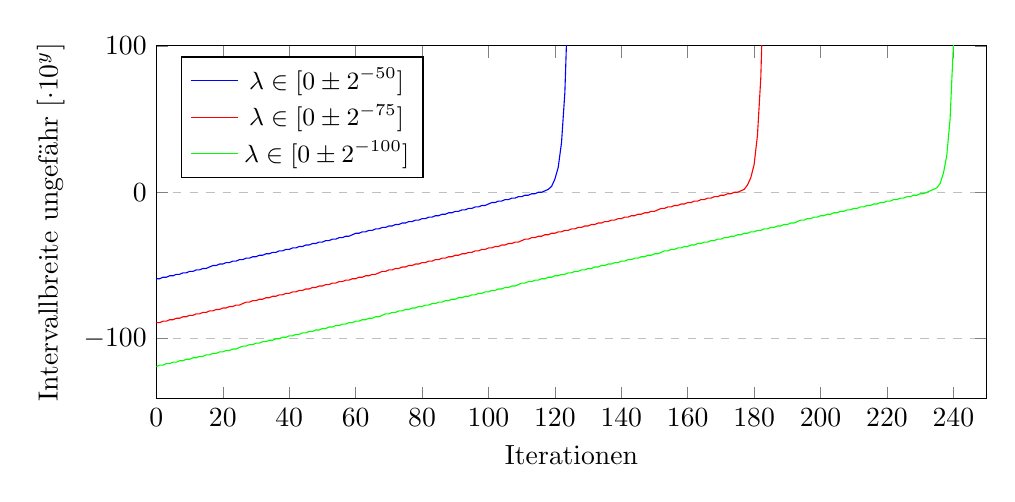
\begin{tikzpicture}
    \begin{axis}[
    width=\textwidth,
    height=0.5\textwidth,
        xlabel={Iterationen},
        ylabel={Intervallbreite ungefähr $[\cdot 10^y ]$},
        legend pos=north west,
        xmin=0,xmax=250,
        ymax=100,
        ymajorgrids=true,
        grid style=dashed,
    ]
    \addplot[
        color=blue,
        ]
        coordinates {
(0,-59) (1,-59) (2,-58) (3,-58) (4,-57) (5,-57) (6,-56) (7,-56) (8,-55) (9,-55) (10,-54) (11,-54) (12,-53) (13,-53) (14,-52) (15,-52) (16,-51) (17,-50) (18,-50) (19,-49) (20,-49) (21,-48) (22,-48) (23,-47) (24,-47) (25,-46) (26,-46) (27,-45) (28,-45) (29,-44) (30,-44) (31,-43) (32,-43) (33,-42) (34,-42) (35,-41) (36,-41) (37,-40) (38,-40) (39,-39) (40,-39) (41,-38) (42,-38) (43,-37) (44,-37) (45,-36) (46,-36) (47,-35) (48,-35) (49,-34) (50,-34) (51,-33) (52,-33) (53,-32) (54,-32) (55,-31) (56,-31) (57,-30) (58,-30) (59,-29) (60,-28) (61,-28) (62,-27) (63,-27) (64,-26) (65,-26) (66,-25) (67,-25) (68,-24) (69,-24) (70,-23) (71,-23) (72,-22) (73,-22) (74,-21) (75,-21) (76,-20) (77,-20) (78,-19) (79,-19) (80,-18) (81,-18) (82,-17) (83,-17) (84,-16) (85,-16) (86,-15) (87,-15) (88,-14) (89,-14) (90,-13) (91,-13) (92,-12) (93,-12) (94,-11) (95,-11) (96,-10) (97,-10) (98,-9) (99,-9) (100,-8) (101,-7) (102,-7) (103,-6) (104,-6) (105,-5) (106,-5) (107,-4) (108,-4) (109,-3) (110,-3) (111,-2) (112,-2) (113,-1) (114,-1) (115,0000) (116,0000) (117,0001) (118,0002) (119,0004) (120,0009) (121,0017) (122,0034) (123,0068) (124,0137) (125,0273) (126,0547) (127,1093) (128,2187) (129,4373) (130,8746)
        };
        \addlegendentry{\small{$\lambda \in [0 \pm 2^{-50}]$}}
        
    \addplot[
        color=red,
        ]
        coordinates {
(0,-89) (1,-89) (2,-88) (3,-88) (4,-87) (5,-87) (6,-86) (7,-86) (8,-85) (9,-85) (10,-84) (11,-84) (12,-83) (13,-83) (14,-82) (15,-82) (16,-81) (17,-81) (18,-80) (19,-80) (20,-79) (21,-79) (22,-78) (23,-78) (24,-77) (25,-77) (26,-76) (27,-75) (28,-75) (29,-74) (30,-74) (31,-73) (32,-73) (33,-72) (34,-72) (35,-71) (36,-71) (37,-70) (38,-70) (39,-69) (40,-69) (41,-68) (42,-68) (43,-67) (44,-67) (45,-66) (46,-66) (47,-65) (48,-65) (49,-64) (50,-64) (51,-63) (52,-63) (53,-62) (54,-62) (55,-61) (56,-61) (57,-60) (58,-60) (59,-59) (60,-59) (61,-58) (62,-58) (63,-57) (64,-57) (65,-56) (66,-56) (67,-55) (68,-54) (69,-54) (70,-53) (71,-53) (72,-52) (73,-52) (74,-51) (75,-51) (76,-50) (77,-50) (78,-49) (79,-49) (80,-48) (81,-48) (82,-47) (83,-47) (84,-46) (85,-46) (86,-45) (87,-45) (88,-44) (89,-44) (90,-43) (91,-43) (92,-42) (93,-42) (94,-41) (95,-41) (96,-40) (97,-40) (98,-39) (99,-39) (100,-38) (101,-38) (102,-37) (103,-37) (104,-36) (105,-36) (106,-35) (107,-35) (108,-34) (109,-34) (110,-33) (111,-32) (112,-32) (113,-31) (114,-31) (115,-30) (116,-30) (117,-29) (118,-29) (119,-28) (120,-28) (121,-27) (122,-27) (123,-26) (124,-26) (125,-25) (126,-25) (127,-24) (128,-24) (129,-23) (130,-23) (131,-22) (132,-22) (133,-21) (134,-21) (135,-20) (136,-20) (137,-19) (138,-19) (139,-18) (140,-18) (141,-17) (142,-17) (143,-16) (144,-16) (145,-15) (146,-15) (147,-14) (148,-14) (149,-13) (150,-13) (151,-12) (152,-11) (153,-11) (154,-10) (155,-10) (156,-9) (157,-9) (158,-8) (159,-8) (160,-7) (161,-7) (162,-6) (163,-6) (164,-5) (165,-5) (166,-4) (167,-4) (168,-3) (169,-3) (170,-2) (171,-2) (172,-1) (173,-1) (174,0000) (175,0000) (176,0001) (177,0002) (178,0005) (179,0010) (180,0019) (181,0039) (182,0078) (183,0156)



        };
        \addlegendentry{\small{$\lambda \in [0 \pm 2^{-75}]$}}
    
        
\addplot[
        color=green,
        ]
        coordinates {
        (0,-119) (1,-118) (2,-118) (3,-117) (4,-117) (5,-116) (6,-116) (7,-115) (8,-115) (9,-114) (10,-114) (11,-113) (12,-113) (13,-112) (14,-112) (15,-111) (16,-111) (17,-110) (18,-110) (19,-109) (20,-109) (21,-108) (22,-108) (23,-107) (24,-107) (25,-106) (26,-105) (27,-105) (28,-104) (29,-104) (30,-103) (31,-103) (32,-102) (33,-102) (34,-101) (35,-101) (36,-100) (37,-100) (38,-99) (39,-99) (40,-98) (41,-98) (42,-97) (43,-97) (44,-96) (45,-96) (46,-95) (47,-95) (48,-94) (49,-94) (50,-93) (51,-93) (52,-92) (53,-92) (54,-91) (55,-91) (56,-90) (57,-90) (58,-89) (59,-89) (60,-88) (61,-88) (62,-87) (63,-87) (64,-86) (65,-86) (66,-85) (67,-85) (68,-84) (69,-83) (70,-83) (71,-82) (72,-82) (73,-81) (74,-81) (75,-80) (76,-80) (77,-79) (78,-79) (79,-78) (80,-78) (81,-77) (82,-77) (83,-76) (84,-76) (85,-75) (86,-75) (87,-74) (88,-74) (89,-73) (90,-73) (91,-72) (92,-72) (93,-71) (94,-71) (95,-70) (96,-70) (97,-69) (98,-69) (99,-68) (100,-68) (101,-67) (102,-67) (103,-66) (104,-66) (105,-65) (106,-65) (107,-64) (108,-64) (109,-63) (110,-62) (111,-62) (112,-61) (113,-61) (114,-60) (115,-60) (116,-59) (117,-59) (118,-58) (119,-58) (120,-57) (121,-57) (122,-56) (123,-56) (124,-55) (125,-55) (126,-54) (127,-54) (128,-53) (129,-53) (130,-52) (131,-52) (132,-51) (133,-51) (134,-50) (135,-50) (136,-49) (137,-49) (138,-48) (139,-48) (140,-47) (141,-47) (142,-46) (143,-46) (144,-45) (145,-45) (146,-44) (147,-44) (148,-43) (149,-43) (150,-42) (151,-42) (152,-41) (153,-40) (154,-40) (155,-39) (156,-39) (157,-38) (158,-38) (159,-37) (160,-37) (161,-36) (162,-36) (163,-35) (164,-35) (165,-34) (166,-34) (167,-33) (168,-33) (169,-32) (170,-32) (171,-31) (172,-31) (173,-30) (174,-30) (175,-29) (176,-29) (177,-28) (178,-28) (179,-27) (180,-27) (181,-26) (182,-26) (183,-25) (184,-25) (185,-24) (186,-24) (187,-23) (188,-23) (189,-22) (190,-22) (191,-21) (192,-21) (193,-20) (194,-19) (195,-19) (196,-18) (197,-18) (198,-17) (199,-17) (200,-16) (201,-16) (202,-15) (203,-15) (204,-14) (205,-14) (206,-13) (207,-13) (208,-12) (209,-12) (210,-11) (211,-11) (212,-10) (213,-10) (214,-9) (215,-9) (216,-8) (217,-8) (218,-7) (219,-7) (220,-6) (221,-6) (222,-5) (223,-5) (224,-4) (225,-4) (226,-3) (227,-3) (228,-2) (229,-2) (230,-1) (231,-1) (232,0000) (233,0001) (234,0002) (235,0003) (236,0006) (237,0013) (238,0025) (239,0050) (240,0101) 


        };
        \addlegendentry{\small{$\lambda \in [0 \pm 2^{-100}]$}}
    
    \end{axis}
    \end{tikzpicture}
    \caption{Größenordnung der Breite des Kernintervalls bei der Berechnung von $x_{250}$ mit Sweeping simple}
    \label{fig:strategy}
\end{figure}

% 
\begin{figure}[ht]
    \centering
    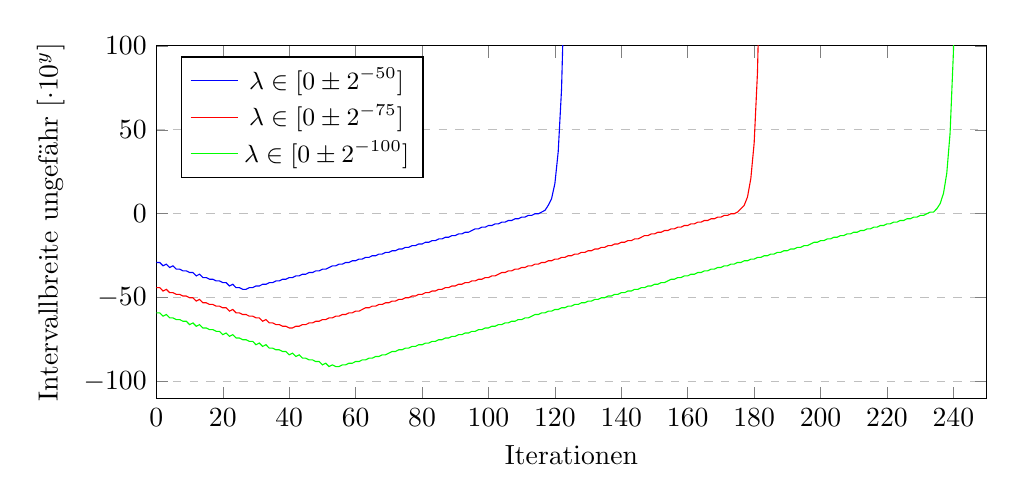
\begin{tikzpicture}
    \begin{axis}[
    width=\textwidth,
    height=0.5\textwidth,
        xlabel={Iterationen},
        ylabel={Intervallbreite ungefähr $[\cdot 10^y ]$},
        legend pos=north west,
        xmin=0,xmax=250,
        ymax=100,
        ymajorgrids=true,
        grid style=dashed,
    ]
    
    \addplot[
        color=blue,
        ]
        coordinates {
 (0,-29) (1,-29) (2,-31) (3,-30) (4,-32) (5,-31) (6,-33) (7,-33) (8,-34) (9,-34) (10,-35) (11,-35) (12,-37) (13,-36) (14,-38) (15,-38) (16,-39) (17,-39) (18,-40) (19,-40) (20,-41) (21,-41) (22,-43) (23,-42) (24,-44) (25,-44) (26,-45) (27,-45) (28,-44) (29,-44) (30,-43) (31,-43) (32,-42) (33,-42) (34,-41) (35,-41) (36,-40) (37,-40) (38,-39) (39,-39) (40,-38) (41,-38) (42,-37) (43,-37) (44,-36) (45,-36) (46,-35) (47,-35) (48,-34) (49,-34) (50,-33) (51,-33) (52,-32) (53,-31) (54,-31) (55,-30) (56,-30) (57,-29) (58,-29) (59,-28) (60,-28) (61,-27) (62,-27) (63,-26) (64,-26) (65,-25) (66,-25) (67,-24) (68,-24) (69,-23) (70,-23) (71,-22) (72,-22) (73,-21) (74,-21) (75,-20) (76,-20) (77,-19) (78,-19) (79,-18) (80,-18) (81,-17) (82,-17) (83,-16) (84,-16) (85,-15) (86,-15) (87,-14) (88,-14) (89,-13) (90,-13) (91,-12) (92,-12) (93,-11) (94,-11) (95,-10) (96,-9) (97,-9) (98,-8) (99,-8) (100,-7) (101,-7) (102,-6) (103,-6) (104,-5) (105,-5) (106,-4) (107,-4) (108,-3) (109,-3) (110,-2) (111,-2) (112,-1) (113,-1) (114,000) (115,000) (116,001) (117,002) (118,005) (119,009) (120,018) (121,037) (122,074) (123,147)
        };
        \addlegendentry{\small{$\lambda \in [0 \pm 2^{-50}]$}}
    
    \addplot[
        color=red,
        ]
        coordinates {
    (0,-44) (1,-44) (2,-46) (3,-45) (4,-47) (5,-47) (6,-48) (7,-48) (8,-49) (9,-49) (10,-50) (11,-50) (12,-52) (13,-51) (14,-53) (15,-53) (16,-54) (17,-54) (18,-55) (19,-55) (20,-56) (21,-56) (22,-58) (23,-57) (24,-59) (25,-59) (26,-60) (27,-60) (28,-61) (29,-61) (30,-62) (31,-62) (32,-64) (33,-63) (34,-65) (35,-65) (36,-66) (37,-66) (38,-67) (39,-67) (40,-68) (41,-68) (42,-67) (43,-67) (44,-66) (45,-66) (46,-65) (47,-65) (48,-64) (49,-64) (50,-63) (51,-63) (52,-62) (53,-62) (54,-61) (55,-61) (56,-60) (57,-60) (58,-59) (59,-59) (60,-58) (61,-58) (62,-57) (63,-56) (64,-56) (65,-55) (66,-55) (67,-54) (68,-54) (69,-53) (70,-53) (71,-52) (72,-52) (73,-51) (74,-51) (75,-50) (76,-50) (77,-49) (78,-49) (79,-48) (80,-48) (81,-47) (82,-47) (83,-46) (84,-46) (85,-45) (86,-45) (87,-44) (88,-44) (89,-43) (90,-43) (91,-42) (92,-42) (93,-41) (94,-41) (95,-40) (96,-40) (97,-39) (98,-39) (99,-38) (100,-38) (101,-37) (102,-37) (103,-36) (104,-35) (105,-35) (106,-34) (107,-34) (108,-33) (109,-33) (110,-32) (111,-32) (112,-31) (113,-31) (114,-30) (115,-30) (116,-29) (117,-29) (118,-28) (119,-28) (120,-27) (121,-27) (122,-26) (123,-26) (124,-25) (125,-25) (126,-24) (127,-24) (128,-23) (129,-23) (130,-22) (131,-22) (132,-21) (133,-21) (134,-20) (135,-20) (136,-19) (137,-19) (138,-18) (139,-18) (140,-17) (141,-17) (142,-16) (143,-16) (144,-15) (145,-15) (146,-14) (147,-13) (148,-13) (149,-12) (150,-12) (151,-11) (152,-11) (153,-10) (154,-10) (155,-9) (156,-9) (157,-8) (158,-8) (159,-7) (160,-7) (161,-6) (162,-6) (163,-5) (164,-5) (165,-4) (166,-4) (167,-3) (168,-3) (169,-2) (170,-2) (171,-1) (172,-1) (173,00) (174,00) (175,01) (176,03) (177,05) (178,10) (179,21) (180,42) (181,84) (182,168)
        };
        \addlegendentry{\small{$\lambda \in [0 \pm 2^{-75}]$}}
    
    \addplot[
        color=green,
        ]
        coordinates {
    (0,-59) (1,-59) (2,-61) (3,-60) (4,-62) (5,-62) (6,-63) (7,-63) (8,-64) (9,-64) (10,-66) (11,-65) (12,-67) (13,-66) (14,-68) (15,-68) (16,-69) (17,-69) (18,-70) (19,-70) (20,-72) (21,-71) (22,-73) (23,-72) (24,-74) (25,-74) (26,-75) (27,-75) (28,-76) (29,-76) (30,-78) (31,-77) (32,-79) (33,-78) (34,-80) (35,-80) (36,-81) (37,-81) (38,-82) (39,-82) (40,-84) (41,-83) (42,-85) (43,-84) (44,-86) (45,-86) (46,-87) (47,-87) (48,-88) (49,-88) (50,-90) (51,-89) (52,-91) (53,-90) (54,-91) (55,-91) (56,-90) (57,-90) (58,-89) (59,-89) (60,-88) (61,-88) (62,-87) (63,-87) (64,-86) (65,-86) (66,-85) (67,-85) (68,-84) (69,-84) (70,-83) (71,-82) (72,-82) (73,-81) (74,-81) (75,-80) (76,-80) (77,-79) (78,-79) (79,-78) (80,-78) (81,-77) (82,-77) (83,-76) (84,-76) (85,-75) (86,-75) (87,-74) (88,-74) (89,-73) (90,-73) (91,-72) (92,-72) (93,-71) (94,-71) (95,-70) (96,-70) (97,-69) (98,-69) (99,-68) (100,-68) (101,-67) (102,-67) (103,-66) (104,-66) (105,-65) (106,-65) (107,-64) (108,-64) (109,-63) (110,-63) (111,-62) (112,-62) (113,-61) (114,-60) (115,-60) (116,-59) (117,-59) (118,-58) (119,-58) (120,-57) (121,-57) (122,-56) (123,-56) (124,-55) (125,-55) (126,-54) (127,-54) (128,-53) (129,-53) (130,-52) (131,-52) (132,-51) (133,-51) (134,-50) (135,-50) (136,-49) (137,-49) (138,-48) (139,-48) (140,-47) (141,-47) (142,-46) (143,-46) (144,-45) (145,-45) (146,-44) (147,-44) (148,-43) (149,-43) (150,-42) (151,-42) (152,-41) (153,-41) (154,-40) (155,-39) (156,-39) (157,-38) (158,-38) (159,-37) (160,-37) (161,-36) (162,-36) (163,-35) (164,-35) (165,-34) (166,-34) (167,-33) (168,-33) (169,-32) (170,-32) (171,-31) (172,-31) (173,-30) (174,-30) (175,-29) (176,-29) (177,-28) (178,-28) (179,-27) (180,-27) (181,-26) (182,-26) (183,-25) (184,-25) (185,-24) (186,-24) (187,-23) (188,-23) (189,-22) (190,-22) (191,-21) (192,-21) (193,-20) (194,-20) (195,-19) (196,-19) (197,-18) (198,-17) (199,-17) (200,-16) (201,-16) (202,-15) (203,-15) (204,-14) (205,-14) (206,-13) (207,-13) (208,-12) (209,-12) (210,-11) (211,-11) (212,-10) (213,-10) (214,-9) (215,-9) (216,-8) (217,-8) (218,-7) (219,-7) (220,-6) (221,-6) (222,-5) (223,-5) (224,-4) (225,-4) (226,-3) (227,-3) (228,-2) (229,-2) (230,-1) (231,-1) (232,00) (233,01) (234,01) (235,03) (236,06) (237,12) (238,24) (239,48) (240,96) (241,192)
        };
        \addlegendentry{\small{$\lambda \in [0 \pm 2^{-100}]$}}
    
    
    
    
    
    
    \end{axis}
    \end{tikzpicture}
    \caption{Größenordnung der Breite des Kernintervalls bei der Berechnung von $x_{250}$ mit Sweeping square\_only}
    \label{fig:strategy2}
\end{figure}


\chapter{Implementierung der Polynome}

Die Implementierung der einzelnen Bestandteile ist objektorientiert. Dieses Kapitel bietet einen Überblick über die Struktur des Programmes und den wichtigsten zu Verfügung stehenden Funktionen.

\section{Darstellung}

\paragraph{Intervalle}
Intervalle enthalten Informationen über deren Zentrum \verb+center+ und Radius \verb+radius+, beziehungsweise deren Breite, welche, je nach gewähltem Zahlentypen, reelle oder rationale Zahlen sind. Zudem können Intervalle ein- oder beidseitig unendlich sein, weshalb wiederum eine Abfrage nach \verb+IntType+\footnote{ FINITE, LOWER\_BOUND, UPPER\_BOUND, ENTIRE }, also dem Intervalltypen möglich ist. Existiert eine Schranke, also ist das Intervall endlich oder einseitig unendlich, kann diese abgefragt werden. \par
Beim Verrechnen von Intervallen sind folgende Regeln zu beachten:
\begin{itemize}
    \item[] $[x_1, x_2] + [y_1, y_2] = [x_1 + y_1, x_2 + y_2]$
    \item[] $[x_1, x_2] - [y_1, y_2] = [x_1 - y_2, x_2 - y_1]$
    \item[] $[x_1, x_2] \cdot [y_1, y_2] = [min(x_1 y_1, x_1 y_2, x_2 y_1, x_2 y_2), max(x_1 y_1, x_1 y_2, x_2 y_1, x_2 y_2)]$
    \item[] $[x_1, x_2] / [y_1, y_2] = [min(x_1 / y_1, x_1 / y_2, x_2 / y_1, x_2 / y_2), max(x_1 /y_1, x_1 /y_2, x_2 /y_1, x_2 /y_2)]$
\end{itemize}
Hier wird der Effekt deutlich, dass Intervalle nach jeder Operation die Tendenz haben, zu wachsen. Wird  bespielsweise ein Intevall  von sich selbst subtrahiert, wird es größer, statt sich wegzukürzen.



\paragraph{Fehlersymbole} 
Ein Fehlersymbol $\lambda$ besteht aus seinem Exponenten, einem \verb+Pointer+ auf das Intervall in dem sein Wert liegt, welches sich während der Berechnung verändern kann und dem Index des Fehlersymbols.

\paragraph{Monome}
Momome werden durch einen Intervallkoeffizienten und eine Liste von nach ihrem Index aufsteigend geordneten Fehlersymbolen dargestellt. Die Implementierung der Liste der Fehlersymbole als \verb+std::vector+, ermöglicht die Verwendung der \textit{C++ Standard Template Library} für Funktionen, wie zum Beispiel die Berechnung des Grades eines Monoms.

\paragraph{Polynome}
Ein Polynom setzt sich aus einem Kernintervall (\verb+kernel+), also dem Monom ohne Fehlersymbole und einer Liste ungleicher Monome zusammen. Ungleich bedeutet in diesem Fall, dass sich die Zusammensetzung  oder der Exponent einzelner Fehlersymbole zwischen den Monomen unterscheidet.


\section{Addition}

Wird wie in \cite{geobuckets} eine Ordnung $\succ$ auf den Monomen definiert, können die Polynome sortiert werden.
\begin{itemize}
    \label{def:order}
    \item $\lambda_1 \succ \lambda_2 \succ...\succ \lambda_k $
    \item $\lambda_n^i \lambda_m^j \succ \lambda_n^{i'} \lambda_m^{j'} $ für $n > m$, falls
    \begin{itemize}
        \item[] $ i > i'$, oder
        \item[] $ i = i'$ und $ j > j'$
    \end{itemize}
\end{itemize}
Diese Ordnung ist partiell, da gleiche Monome, beziehungsweise Monome mit gleichen Fehlersymbolen nicht vergleichbar sind. Tritt dieser Fall während der Addition zweier Polynome auf, bedeutet das, dass die Koeffizienten beider Monome addiert werden und das so entstandene Monom in die Polynom-Summe aufgenommen wird.
Haben die verglichenen Monome die selbe Anzahl an Variablen, entscheidet die Größe des Exponenten des Fehlersymbols mit dem kleinsten Index. Algorithmus \ref{algo:maxes} implementiert diese Ordnung und hat den Vorteil, dass nicht immer alle Fehlersymbole aus beiden Listen betrachtet werden müssen. Sobald sich die beiden Monome, genauer deren Fehlersymbole, an der ersten Stelle unterscheiden, terminiert die Schleife. Die Vorbedingung hierfür ist, dass die Fehlersymbole in den Listen aufsteigend sortiert sind.


In vorhergegangen Implementierungen der Fehlersymbole waren diese noch keine Objekte. Stattdessen hatte jedes Monom einen \verb vector  mit einem Eintrag pro Fehlersymbol. Der Index des Fehlersymbol entsprach dem Index innerhalb des Vectors, der Wert im \verb vector  dem Exponenten, was die Datenstruktur vereinfachte, aber erforderte, dass alle Monome dieselbe Anzahl an Fehlersymbolen hatten. Da sich diese allerdings ändern kann, wenn durch ein \verb Polish  ein neues $\lambda$ hinzugefügt oder eines der $\lambda$s durch \verb Sweeping  kein Vorkommen mehr hat und entfernt werden kann, wurde eine andere Herangehensweise verwendet.


\begin{algorithm}[H]
\label{algo:maxes}
\SetAlgoLined
\SetKwInOut{Input}{input}
\Input{Zwei Listen von Fehlersymbolen $ess_1, ess_2$}
$size \gets max\{length(ess_1), length(ess_2)\}$\; 
$i \gets 0 $ \;
\While{i < size}{
  \uIf{$i \geq length(ess_1)\ \textbf{or}\ ess_1[i] \succ ess_2[i]$}{
        \Return right
  }\uElseIf{$i \geq length(ess_2)\ \textbf{or}\ ess_1[i] \prec ess_2[i]$}{
        \Return left
  }
}
\Return equal
 \caption{max\_errorsymbols}
\end{algorithm}

Werden nun sortierte Polynome $p_1, p_2$ addiert, geschieht lediglich ein Zusammenführen (merge) zweier geordneter Listen, was im schlimmsten Fall $\#p_1 + \#p_2$ Vergleiche der Monome benötigt\footnote{$\#p$ liefert die Anzahl an Monomen des Polynoms $p$}. 

 
\begin{algorithm}[H]
\SetAlgoLined
\label{algo:add}
\SetKwInOut{Input}{input}
\Input{Polynome $p_1, p_2$}
$p \gets (), i \gets 0, j \gets 0$ \; 
\While{$i < \#p_1$ \textbf{and} $j  < \#p_2$} {
    $max \gets max\_errorsymbols(p_1[i], p_1[j])$ \;
    \uIf{max = left}{
        $p.append(p_1[i])$\;
        $i \gets i+1 $\;
    }
    \uElseIf{max = right}{
        $p.append(p_2[j])$\;
        $j \gets j+1 $\;
    }
    \uElse{ // $max = equal$\\
        $p.append(p_1[i] + p_1[j])$\;
        $p_1.remove(i)$\;
        $i \gets i+1; j \gets j +1 $\;
    }
}
Append the rest to $p$\;
\Return $p$

 \caption{Addition zweier Polynome}
\end{algorithm}

Algorithmus \ref{algo:add} erzeugt aus zwei nach der oben definierten Ordnung $\prec$ sortierten Polynomen wiederum ein sortiertes Polynom. Endet die While-Schleife in Zeile 2, so ist im Regelfall eines der Polynome noch nicht gänzlich betrachtet, was bedeutet, dass alle übrigen Monome in diesem Polynom (im Hinblick auf $\prec$) kleiner sind, als die des anderen Summanden und daher dem Ergebnispolynom angehangen werden können, ohne sie weiter zu betrachten. 



\section{Multiplikation}
In einer linearen Implementierung der Taylormodelle wird bei der Multiplikation immer eines der Fehlersymbole gesweept, sodass die Länge eines Polynoms nicht über die Dimension hinausgeht und somit der Schwerpunkt bei der Intervallarithmetik liegt. Lässt man allerdings höhere Ordnungen zu, werden auch die Polynome länger und ein Weiteres Problem tritt auf. Um die oben (\ref{def:order}) definierte Ordnung $\prec$ auf dem Polynom $p = p_1 \cdot p_2$ zu erhalten, müssen die $n\cdot m$ Monome ($n := \#p_1, m := \#p_2$), die bei der Multiplikation entstehen sortiert werden. Werden diese sequentiell zu $p$ hinzugefügt bedeutet das 2 Vergleiche, dann 3, dann 4, und so weiter, bis hin zu $nm$ Vergleichen:
$$ 2 + 3 + 4 + 5 + ... + nm = \frac{nm \cdot (nm + 1)}{2} - 1$$
So ergibt sich für die naive Multiplikation eine quadratische Laufzeit in $O$-Notation von $O(nm + (nm)^2)$
\par
Für effizientere Polynommultiplikation existieren verschiedene Algorithmen. Viele der schnellen bekannten Algorithmen basieren  auf der Schnellen-Fourier-Transformation, wobei die Polynome in Stützvektoren und wieder zurück umgewandelt werden. Da es sich bei den Koeffizienten den Monome um Intervalle mit möglicherweise unendlichen Schranken handelt, ist das Rückführen eines Stützvektors nicht immer ohne Weiteres möglich. (TODO Nachgucken FFT Intervallartihmetik) \par
Ein Weiterer Ansatz besteht darin, die Anzahl der benötigten Monomvergleiche zu reduzieren, wenn die Monome einsortiert werden müssen. Betrachtet man die Summe dreier Polynome $p_1 + p_2 + p_3$ mit $\#p_1 >> \#p_2 = \#p_3 = 1$, benötigt das Aufsummieren von links nach rechts $2\#p_1 + 1$ Vergleiche, da mit dem oben verwendeten Additionsverfahren zweifach in $p_1$ eingefügt wird. Summiert man jedoch von rechts nach links so werden lediglich $\#p_1 + 2$ Vergleiche benötigt. Nach dieser Idee kann die Anzahl der Monomvergleiche reduziert werden, indem zunächst Polynome gleicher Länge miteinander addiert werden. Mit Geobuckets, von Yan (\cite{geobuckets}) eingeführt und Monagan und Pearce (\cite{geobucketsmulti}) für die Multiplikation angepasst, werden die Zwischenergebnisse der Polynommultiplikation in geometrisch wachsenden 'Buckets' gespeichert. Hat ein Bucket seine Kapazität erreicht, wird das Polynom zum nächst größeren Bucket hinzuaddiert. Der Unterschied zum Originalalgorithmus besteht darin, dass die Größe der hinzukommenden Polynome bereits kennt und die Bucketkapazität dementsprechend anpassen kann. Algorithmus \ref{algo:mult} zeigt die in \verb+hotm+ implementierte Version der Geobucketmultiplikation. Durch den Teile und Herrsche Ansatz, kann die Multiplikation mit Geobuckets in $O(nm \log nm)$ durchgeführt werden.  \par
Sei $x_0 = 0.5 + 1 \lambda_1 + 1 \lambda_2 + 1 \lambda_3$ und einem Startfehler von $2^{-21}$, also $\lambda_i \in [0 \pm 2^{-20}]\text{ für }i \in \{1,2,3\}$. Berechnet man nun $x_{i+1} = 3.75 \cdot x_i \cdot (1 - x_i)$ zeigen sich deutliche Unterschiede bei den benötigten Monomvergleichen, beziehungsweise dem Aufruf der Funktion \verb+max_monomial+  (Algorithmus \ref{algo:maxes}).

\begin{table}[ht]
    \centering
    \def\arraystretch{1.3}
    \begin{tabular}{c|c|c}
    \multicolumn{3}{l}{\makecell{Naive Multiplikation}} \\
    \hline
    Grad nach Reduktion & CPU-Zeit & \#Vergleiche \\
    5 & 2.375 s&  $\approx 1.3 \cdot 10^7 $\\
    6 & 5.281 s&  $\approx 4 \cdot 10^7 $\\
    7& 11.281 s&  $\approx 1 \cdot 10^8 $\\
    8& 22.406 s s&  $\approx 2.2 \cdot 10^8 $\\
    \hline
    \multicolumn{3}{l}{\makecell{Multiplikation mit Geobuckets}} \\
    \hline 
    Grad nach Reduktion & CPU-Zeit & \#Vergleiche \\
    5 & 1.875 s&  $\approx 3\cdot 10^5$\\
    6 & 3.859 s&  $\approx 1 \cdot 10^6 $\\
    7 & 6.406 s&  $\approx 1.8 \cdot 10^6 $\\
    8 & 11.14 s&  $\approx 3.3 \cdot 10^6 $\\
    \end{tabular}
    \caption[Multiplikation: Geobuckets gegen Naiv]{Berechnung von $x_{10}$ mit Reduzierung des Grades nach jeder Iteration. Gemessen mit dem iRRAM-internen Debugmodus und Code-Coverage.}
    \label{tab:my_label}
\end{table}

\begin{figure}
    \centering
    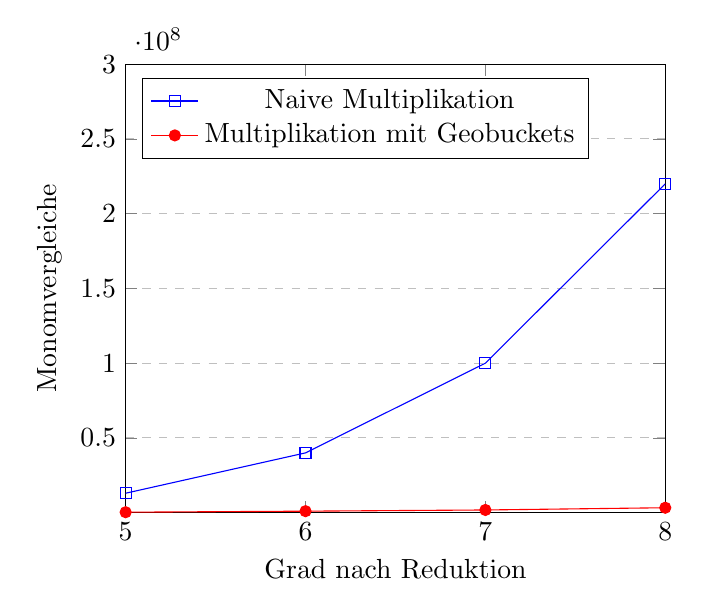
\begin{tikzpicture}
    \begin{axis}[
        xlabel={Grad nach Reduktion},
        ylabel={Monomvergleiche},
        xmin=5, xmax=8,
        ymin=100000, ymax=300000000,
        xtick={5,6,7,8},
        legend pos=north west,
        ymajorgrids=true,
        grid style=dashed,
    ]
    \addplot[
        color=blue,
        mark=square
        ]
        coordinates {
        (5, 13000000)(6, 40000000 )(7, 100000000)(8, 220000000)
        };
        \addlegendentry{Naive Multiplikation}
        
    \addplot[
        color=red,
        mark=*
        ]
        coordinates {
        (5, 300000)(6, 1000000 )(7, 1800000)(8, 3300000)
        };
        \addlegendentry{Multiplikation mit Geobuckets}
    
    \end{axis}
    \end{tikzpicture}
    \label{fig:my_label}
    \caption{Naive Multiplikation gegen Multiplikation mit Geobuckets}
\end{figure}





\begin{algorithm}
\SetAlgoLined
\label{algo:mult}
\SetKwInOut{Input}{input}
\Input{Polynome $p_1, p_2$}
// Initialize \\
$n \gets \#p_1, m\gets \#p_2$ \;
$p \gets [\ ]$ \;
Allocate $buckets$ with space for polynomials: $\{2m, 4m, ..., 2^{\lceil log_2(n)\rceil -1 }m\}$\;
$i\gets 0 $\;
// Main Loop \\
\While{$i < n$}{
    $p \gets p_1[i] \cdot p_2$\;
    \uIf{$i < (n-1)$}{
        $p \gets p + p_1[i+1] \cdot p_2$\;
    }
    $i\gets i+2$\;
   $j\gets 0 $\; 
    \While{$buckets[j].not\_empty()$}{
        $p \gets p + buckets[j]$ \;
        $buckets[j] \gets [\ ]$\;
        $j\gets j+1 $\; 
    }
    \uIf{$i < n$}{
        $buckets[j] \gets p$\;
        $p \gets [\ ]$ \;
    }
    
}
// Merge each bucket into the final polynomial\\
\ForEach{$bucket \in buckets$}{
    $p \gets p + bucket$\;
}


\Return $p$

 \caption{Polynommultipliaktion mit Geobuckets}
\end{algorithm}

\chapter{iRRAM}
Die Software-Bibliothek \verb+iRRAM+ \cite{Mller2009EnhancingIE} basiert auf Intervallen als Zahlentyp, um diese mit einer beliebigen Genauigkeit darstellen zu können. Zunächst wird mit Double-Präzision (64-Bit Zahlen) gerechnet, welche verwendet werden, bis das Ergebnis für die angefragte Präzision nicht mehr genau ausgegeben werden kann, beziehungsweise bis zu einer bestimmten Anzahl an Bits. Ist dies der Fall, geschieht eine Iteration mit einer erhöhten Genauigkeit, also längeren Zahlen, welche dann mit Hilfe von \verb+MPFR+ dargestellt werden.
Für eine solche Iteration werden gerade so viele Zwischenergebnisse während der Berechnung gespeichert, dass eine Wiederholung der Schritte mit höherer Präzision möglich ist. Da nicht die gesamte Berechnung in jeder Iteration wiederholt wird, müssen während der Laufzeit Sichtbarkeit von Variablen und Zwischenergebnisse für den Nutzer genau kontrolliert und unter Umständen beschränkt werden, da sonst unerwartetes Verhalten und Exceptions entstehen können, indem die zugegriffenen Werte gegebenfall nicht in der aktuellen Iteration existieren.

\section{Verwendung der iRRAM-REALs}
Einige der für rationale Zahlen zur Verfügung stehenden Funktionen, wie der Vergleich zweier Zahlen, sind mit reellen Zahlen nicht ohne Weiteres Möglich. Dies gilt insbesondere für den Test auf Gleichheit und die Vorzeichenfunktion $sign$. Bei all diesen Funktionen handelt es sich im Reellen (und bei der \verb+iRRAM+) um mehrwertige Funktionen, da sich das jeweilige Ergebnis mit veränderter Präzsion in der Darstellung der Zahlen ändern kann. Dieses Problem wird in \verb+hotm+ durch den \verb+SignType+ adressiert. Zusätzlich zu den Werten 'positiv' (=\verb+POS+) und 'negativ' (=\verb+NEG+),  kann die Vorzeichenfunktion \verb+sign+ den Wert 'ambivalent' (=\verb+AMBI+) ausgeben, wenn nicht entscheidbar ist, wo genau die reelle Zahl um die Null liegt. Hierfür erhält die Vorzeichenfunktion einen Parameter, der den Bereich er Unsicherheit definiert. Ist der Ausgabewert 'ambivalent', so wird in den Funktionen, welche die Vorzeichenfunktion aufrufen, der schlechteste Fall im Hinblick auf die Genauigkeit des Ergebnisses angenommen. 


Eine weitere Besonderheit ergibt sich aus dem Aufbau der Zahlen, denn es entstehen zwei Intervall-`Ebenen`: Zum Einen, die Darstellung des Koeffizienten als Intervall aus Mitte und Radius. Zum Anderen die Darstellung von Mitte und Radius, als \verb+iRRAM-REAL+, also auch wiederum jeweils als Intervall mit Wert und Fehler, wie in Grafik \ref{fig:levels} zu sehen ist. Im Vergleich zu den \verb+mpq-RATIONALS+ erhöht sich hier zwar die Komplexität deutlich, allerdings lassen sich Ungenauigkeiten sehr genau steuern, indem zum Beispiel der Rechenfehler des Mittelpunkts eines Koeffizienten auf den Radius 'verlagert' wird. So vergrößert sich zwar der Radius des Koeffizienten, welcher dadurch ungenauer wird, jedoch verkleinert sich der Rechenfehler auf der Zahlenebene der \verb+REAL+s. Ein ählicher Effekt sollte sich durch Rundung auch mit den \verb+mpq-RATIONALS+ erreichen lassen. 


Das Verlagern der Ungenauigkeit ($e$ in der Grafik \ref{fig:levels}) auf den Wert des Radius' ($v$ in der Grafik), \textit{Micro-Housekeeping} genannt, verringert die Intervallbreite und erzeugt Punktintervalle auf der Zahlenebene, allerdings werden die Intervalle auf der Intervallebene breiter. Hier greift dann wiederum der Polish-Mechanismus, der auf Polynomebene Monome hinzufügt, um aus den zu groß gewordenen Intervallen wiederum Punktintervalle zu machen, \textit{Macro-Housekeeping} genannt. So wird der Rechenfehler von der untersten Ebene bis zur Polynomebene propagiert.
Diese Housekeeping-Funktionen werden durch Parameter gesteuert, die bestimmen, ab wann ein Intervall zu breit ist und die jeweilige Prozedur angewandt werden soll.

\begin{figure}[ht]
\label{fig:levels}
\begin{center}
 
 

\tikzset{every picture/.style={line width=0.75pt}} %set default line width to 0.75pt        

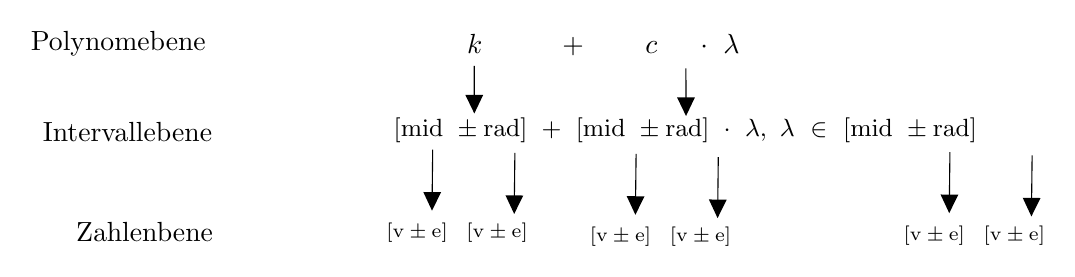
\begin{tikzpicture}[x=0.75pt,y=0.75pt,yscale=-1,xscale=1]
%uncomment if require: \path (0,300); %set diagram left start at 0, and has height of 300

%Straight Lines [id:da29898159624783616] 
\draw    (281.07,90.5) -- (280.77,116.88) ;
\draw [shift={(280.73,119.88)}, rotate = 270.65] [fill={rgb, 255:red, 0; green, 0; blue, 0 }  ][line width=0.08]  [draw opacity=0] (8.93,-4.29) -- (0,0) -- (8.93,4.29) -- cycle    ;
%Straight Lines [id:da1335093356184387] 
\draw    (320.67,92.1) -- (320.37,118.48) ;
\draw [shift={(320.33,121.48)}, rotate = 270.65] [fill={rgb, 255:red, 0; green, 0; blue, 0 }  ][line width=0.08]  [draw opacity=0] (8.93,-4.29) -- (0,0) -- (8.93,4.29) -- cycle    ;
%Straight Lines [id:da1340726243132735] 
\draw    (379.07,92.5) -- (378.77,118.88) ;
\draw [shift={(378.73,121.88)}, rotate = 270.65] [fill={rgb, 255:red, 0; green, 0; blue, 0 }  ][line width=0.08]  [draw opacity=0] (8.93,-4.29) -- (0,0) -- (8.93,4.29) -- cycle    ;
%Straight Lines [id:da9182990047680641] 
\draw    (418.67,94.1) -- (418.37,120.48) ;
\draw [shift={(418.33,123.48)}, rotate = 270.65] [fill={rgb, 255:red, 0; green, 0; blue, 0 }  ][line width=0.08]  [draw opacity=0] (8.93,-4.29) -- (0,0) -- (8.93,4.29) -- cycle    ;
%Straight Lines [id:da04610901450657834] 
\draw    (530.27,91.7) -- (529.97,118.08) ;
\draw [shift={(529.93,121.08)}, rotate = 270.65] [fill={rgb, 255:red, 0; green, 0; blue, 0 }  ][line width=0.08]  [draw opacity=0] (8.93,-4.29) -- (0,0) -- (8.93,4.29) -- cycle    ;
%Straight Lines [id:da7044032296577734] 
\draw    (569.87,93.3) -- (569.57,119.68) ;
\draw [shift={(569.53,122.68)}, rotate = 270.65] [fill={rgb, 255:red, 0; green, 0; blue, 0 }  ][line width=0.08]  [draw opacity=0] (8.93,-4.29) -- (0,0) -- (8.93,4.29) -- cycle    ;
%Straight Lines [id:da7628093943540135] 
\draw    (301.07,50.1) -- (301.12,70.08) ;
\draw [shift={(301.13,73.08)}, rotate = 269.84000000000003] [fill={rgb, 255:red, 0; green, 0; blue, 0 }  ][line width=0.08]  [draw opacity=0] (8.93,-4.29) -- (0,0) -- (8.93,4.29) -- cycle    ;
%Straight Lines [id:da9018979196177348] 
\draw    (403.07,51.3) -- (403.12,71.28) ;
\draw [shift={(403.13,74.28)}, rotate = 269.84000000000003] [fill={rgb, 255:red, 0; green, 0; blue, 0 }  ][line width=0.08]  [draw opacity=0] (8.93,-4.29) -- (0,0) -- (8.93,4.29) -- cycle    ;

% Text Node
\draw (86.2,32) node [anchor=north west][inner sep=0.75pt]   [align=left] {Polynomebene};
% Text Node
\draw (92,76) node [anchor=north west][inner sep=0.75pt]   [align=left] {Intervallebene};
% Text Node
\draw (108,124) node [anchor=north west][inner sep=0.75pt]   [align=left] {Zahlenbene};
% Text Node
\draw (296.4,33.8) node [anchor=north west][inner sep=0.75pt]    {$k\ \ \ \ \ \ \ \ +\ \ \ \ \ \  c\ \ \ \ \cdot \ \lambda $};
% Text Node
\draw (261,74) node [anchor=north west][inner sep=0.75pt]  [font=\small]  {$\left[\text{mid} \ \pm \text{rad}\right] \ +\ \left[\text{mid} \ \pm \text{rad}\right] \ \cdot \ \lambda ,\ \lambda \ \in \ \left[\text{mid} \ \pm \text{rad}\right]$};
% Text Node
\draw (257.5,124.6) node [anchor=north west][inner sep=0.75pt]  [font=\scriptsize]  {$\left[\text{v} \pm \text{e}\right] \ \ \left[\text{v} \pm \text{e}\right]$};
% Text Node
\draw (355.5,126.6) node [anchor=north west][inner sep=0.75pt]  [font=\scriptsize]  {$\left[\text{v} \pm \text{e}\right] \ \ \left[\text{v} \pm \text{e}\right]$};
% Text Node
\draw (506.7,125.8) node [anchor=north west][inner sep=0.75pt]  [font=\scriptsize]  {$\left[\text{v} \pm \text{e}\right] \ \ \left[\text{v} \pm \text{e}\right]$};


\end{tikzpicture}

 \caption{Ebenen der Polynomdarstellung mit REALs (informell)}
 \end{center}
\end{figure}


\section{Genauigkeitsmodell}
Die \verb+iRRAM+ bietet die Möglichkeit, zwischen \textit{absoluter} und \textit{relativer} Genauigkeit zu unterscheiden. Absolute Genauigkeit bedeutet, dass beim Verrechnen zweier \verb+REAL+s ein global verwendeter Wert für die Genauigkeit zugrunde liegt und die Zahlen dementsprechen skaliert werden. Bei relativer Genauigkeit hängt die verwendete Genauigkeit von der tatsächlichen Größe der jeweiligen Zahlen ab. Diese kann zum Beispiel durch punktuelle Anwendung von Micro-Housekeeping stark variieren, weshalb die Verwendung von relativer Genauigkeit in der Praxis besser funktioniert.


Für der Vergleich wurde $x_{1000}$ mit $x_n = c \cdot x_{n-1} \cdot (1 - x_{n-1})$ mit der folgenden Konfiguration berechnet:
\begin{enumerate}
 \item Nur quadratisches Sweeping zur 0,
 \item Micro-Housekeeping (Cleaning) ab einem Fehler auf Zahlenebene $>10^{-100}$,
 \item Macro-Housekeeping (Polish) ab einer Intervallbreite $>10^{-50}$,
 \item $x_0 = 0,5$ und
 \item Ausgabe des Ergebnisses auf 20 Stellen genau.
\end{enumerate}
Zu Beginn einer jeden Iteration wird zunächst gesweept (1.), dann der Fehler und die Intervalle bereinigt (2.) und zuletzt das Polynom poliert (3.), bevor erneut multipliziert wird. Für $c = 3.25$ konvergiert die Funktion gegen zwei Werte und lässt sich sehr genau bestimmen.

\begin{center}
\begin{tabular}{|r|c|c|}
\hline
\multicolumn{3}{|c|}{$c=3.25$}\\
\hline
 ohne Housekeeping&relative Genauigkeit & absolute Genauigkeit \\
 \hline
 \hline
 Anzahl Polishs & 142 & 6961 \\
 Präzision (Bits) & \verb+double+ & 136 \\
 CPU-Zeit & 0.8s & 4.43s\\
 \hline
\end{tabular}
\end{center}

Wie in der Tabelle zu sehen ist, benötigt die Berechnung mit relativer Genauigkeit erheblich weniger Zeit und Bits um ein Ergebnis mit der geforderten Auflösung zu erhalten. Wird auf die Housekeeping-Methoden verzichtet, zeigt sich dieser massive Unterschied jedoch nicht:

\begin{center}
\begin{tabular}{|r|c|c|}
\hline
\multicolumn{3}{|c|}{$c=3.25$}\\
\hline
 ohne Housekeeping &relative Genauigkeit & absolute Genauigkeit \\
 \hline
 \hline
 Anzahl Polishs & -& -\\
 Präzision (Bits) & 7440 & 7440 \\
 CPU-Zeit & 0.120s & 0.118s\\
 \hline
\end{tabular}
\end{center}

Die Ergenisse werden erheblich schneller berechnet, allerdings auf Kosten der benötigten Bits für die Zahlendarstellung. Da hier kein Polieren geschieht, wird auch kein Taylormodell als solches initialisiert, das heißt, es werden keine Fehlersymbole eingesetzt und rein auf der Ebene der reellen Zahlen der \verb+iRRAM+ gerechnet.

Für $c=3.75$, einem Wert, bei dem die Funktion chaotisches Verhalten aufweist und zwischen vielen Werten hin- und herspringt, ist erkennbar, dass ein Rechnen mit diesen Housekeeping-Parametern und absoluter Genauigkeit nicht praktikabel ist, da die Berechnung bereits nach 64 Iterationen eine Laufzeit von über 15 Sekunden hat, welche scheinbar exponentiell steigt:

\begin{center}
\begin{tabular}{|r|c|c|}
\hline
\multicolumn{3}{|c|}{$c=3.75$}\\
\hline
 mit Housekeeping &relative Genauigkeit & absolute Genauigkeit \\
 \hline
 \hline
 Anzahl Polishs & 5511 & ?\\
 Präzision (Bits) & 7440 & ?\\
 CPU-Zeit & 4.02s & >60s\\
 \hline
\end{tabular}
\end{center}

Wie oben zeigt sich zwischen relativer und absoluter Genauigkeit bei der Verwendung ohne Housekeeping-Methoden kein nennenswerter Unterschied. Zudem scheint bei der hier verwendeten Konfiguration lediglich ein Berechnungsoverhead zu entstehen, welcher keine Auswirkungen auf die Qualität des Ergebnisses hat.


\begin{center}
\begin{tabular}{|r|c|c|}
\hline
\multicolumn{3}{|c|}{$c=3.75$}\\
\hline
 ohne Housekeeping &relative Genauigkeit & absolute Genauigkeit \\
 \hline
 \hline
 Anzahl Polishs & - & -\\
 Präzision (Bits) & 7440 & 7440\\
 CPU-Zeit & 0.12s & 0.12s\\
 \hline
\end{tabular}
\end{center}


Insgesamt lässt sich beobachten, dass die Berechnung der Interationen mit relativer Genauigkeit die besten Ergebnisse liefert, weshalb diese im Folgenden zugrunde liegt.

\section{Housekeeping}

% 
% \begin{table}[ht]
%     \centering
%     \def\arraystretch{1.3}
%     \begin{tabular}{r|c|c|c}
%     Iterationen &Metrik & absolut & relativ \\
%     \hline
%     $n=60$ & CPU-Zeit & $0.08s$ &  $3.21s$       \\
%            & Genauigkeit & \verb+double+ &   $2^{-748}$      \\
%            & Anzahl Polishs & 45 &    374     \\ 
%     \hline
%     $n=65$ & CPU-Zeit & $0.14s$ &  $18.06s$       \\
%            & Genauigkeit & \verb+double+ &  $2^{-748}$       \\
%            & Anzahl Polishs & 71 &   409      \\
%     \hline
%     $n=66$ & CPU-Zeit & $0.18s$ & $69s$\\
%            & Genauigkeit & \verb+double+ &   $2^{-748}$      \\
%            & Anzahl Polishs & 77 &    416     \\
%     \hline
%     $n=67$ & CPU-Zeit & $0.23s$ & $180s$ \\
%            & Genauigkeit & \verb+double+ &   $2^{-748}$      \\
%            & Anzahl Polishs & 84 &     423    \\
%     \hline
%     $n=100$ & CPU-Zeit & $0.38s$ & $>180s$ \\
%            & Genauigkeit & $2^{-748}$ &??\\
%            & Anzahl Polishs & 314 &??\\
%     \hline
%     $n=500$ & CPU-Zeit & $2.83s$ &$>180s$\\
%            & Genauigkeit & $2^{-2876}$ &??\\
%            & Anzahl Polishs & 3939 &??\\
%     \end{tabular}
%     \caption[Vergleich von Genauigkeitsmodellen]{Vergleich vom Rechnen mit absoluter und relativer Genauigkeit}
%     \label{tab:precision}
% \end{table}

% %% eval.tex
%% $Id: eval.tex 61 2012-05-03 13:58:03Z bless $

\chapter{Evaluation}
\label{ch:Evaluierung}
%% ==============================

Werden die Initialwerte für Iterationen der H\e non-Abbildung $(x_0, y_0)$ als Taylormodelle mit Itervallen definiert, kann eine Fläche beschrieben werden, die durch die Abbildung gespiegelt, gedehnt und verzerrt wird. Liegt diese für $a=1.4$ und $b=0.3$ komplett innerhalb der Fangzone $R$, so wird jeder Punkt in der Fläche wiederum nach $R$ abgebildet. 

\Abbildungps{tbh}{.7}{img/6iter.pdf}{fig:escape}{H\e non-Abbildung: Mehrere Iterationen mit großen Initialwerten}{Iterationen der H\e non-Abbildung ausgehend von einem größeren Rechteck}

Eine Abbildung der Fläche im Ganzen führt jedoch zu einer Überschätzung, die in jeder Iteration zunimmt, da nun mit Intervallen statt mit Punkten gerechnet wird. Abbildung \ref{fig:escape} zeigt pro Graph eine Iteration mit 
\begin{align*}
x_0 = 0 + 1 \cdot \lambda_1 & \hspace{0.5cm} (\lambda_1 \in [0 \pm 0.4]) \\
 y_0 = 0 + 1 \cdot \lambda_2 & \hspace{0.5cm} (\lambda_2 \in [0 \pm 0.1])
\end{align*}
und der Fangzone als schwarzes Tetragon. Es ist erkennbar, dass das Rechteck nach wenigen Iterationen die Fangzone verlässt und einige Itervalle ein starkes Rauschen verursachen. Abbildung \ref{fig:7iter} zeigt  Iterationen mit kleineren initialen Intervallen, wodurch die Überschätzung erst zu einem späteren Zeitpunkt zu groß wird. Um dem Wachstum der Intervalle entgegenzuwirken und die Berechnung der H\e non-Abbildung auch für solche Flächem mit höheren Iterationszahlen zu ermöglichen, könnten die Taylormodelle in Partitionen aufgeteilt werden.  Die kleinste Partitionierung wäre die Aufteilung der Fläche in unendlich viele Punkte, was nicht praktikabel wäre, allerdings hohe Iterationszahlen ermögliche, wie in Abbildung \ref{fig:strangeattractor} zu sehen ist. Das andere Extrem stellen große Itervalle, beziehungsweise keine Partitionierung dar, was im Vergleich nur einen Bruchteil des Rechenaufwandes bedeutet, jedoch schnell zu starker Überschätzung führt.

In diesem Kapitel wird untersucht, wie sich die \verb+HOTM+ bei verschiedenen Intervallgrößen verhalten und welche Konfiguration der Parameter für die Housekeeping-Methoden und den Taylormodellen selbst zu einer möglichst kleinen Überschätzng führt.
Der Housekeeping-Vorgang der in jeder Iteration bei den Taylormodellen angwandt wird besteht aus vier Schritten:
 \begin{enumerate}
  \item \textbf{(Sweeping)} Reduktion des Taylormodells bis zum angegebenen Grad, je nach Strategie
  \item \textbf{(Sweeping überschüssiger Fehlersymbole)} Entfernen aller Fehlersymbole bis auf die $n$-größten (abhängig von deren Support-Space)
  \item \textbf{(Cleaning)} Verlagern der durch die Schritte 1 und 2 entstandenen Rechenfehler auf der Ebene der \verb+iRRAM-REAL+s auf die Radii der Intervalle
  \item \textbf{(Splitting)} Einführen neuer Fehlersymbole für Monome, deren Koeffizienten durch die Schritte 1-3 zu stark gewachsen sind.
 \end{enumerate}

% Um die Fragestellung, wie die H\e non-Abbildung mit Taylormodellen am besten berechnet werden kann zu erörtern, wird das Problem in drei Sektionen unterteilt:
% 
% \begin{enumerate}
%  \item Wie klein müssen die Taylormodelle sein, damit längere Berechnungen möglich sind?
%  \item Wie verhalten sich die verschiedenen Partitionsgrößen bei unterschiedlichen Konfigurationen der Taylormodelle?
%  \item Welche Partition ist für eine gegebene Anzahl an Iterationen nötig?
% \end{enumerate}
% 



Die Implementierung nichtlinearer Taylormodelle ergibt eine Vielzahl von Konfigurationsmöglichkeiten und damit einen großen Suchraum nach der optimalen Einstellung:
\begin{itemize}
 \item Grenzwert für Cleaning $\delta_c$, Splitting $\delta_s$
 \item Grad der Reduktion durch Sweeping
 \item Anzahl der zu erhaltenden Fehlersymbole
 \item Strategie beim Sweeping
 \item Heuristik für die Reihenfolge, in der Fehlersymbole gesweept werden
 \item Vorgehen beim Splitting
 \item Definition des initialen Taylormodells
\end{itemize}
Diese Konfigurationen können in \verb+HOTM+ als JSON-Datei mit Hilfe einer JSON-Bibliothek\footnote{\url{https://github.com/nlohmann/json} (Stand Dezember 2020)} eingelesen und verarbeitet werden, um wiederholte Durchläufe mit leicht veränderten Parametern oder Batch-Runs zu vereinfachen. Listing \ref{list:config} zeigt ein Beispiel einer Konfigurationsdatei, mit der versuchsweise 1000 Iterationen der H\e non-Abbildung berechnet werden sollen. 



\section{Housekeeping-Grenzwerte}
Der Grenzwert einer Housekeeping-Methode gibt an ab welchem Wert die jeweilige Methode angewandt wird. Bei einem intervall in \verb+HOTM+ $I=[m \pm r]$ mit $m = [c_m \pm \varepsilon_m]$ und $r = [c_r \pm \varepsilon_r]$ als \verb+iRRAM-REAL+s wird
\begin{itemize}
 \item Cleaning angewandt, wenn $\varepsilon_m < \delta_c$ oder $\varepsilon_r < \delta_c$ gilt und
 \item Splitting angewandt, wenn $c_m < \delta_s$ oder $c_m < \delta_s$ gilt.
\end{itemize}
Um diese Werte zu untersuchen, wurde betrachtet, wie sich die Größe des Rechtecks, welches durch die Intervalle $x$ und $y$ aufgespannt wird, abhängig von den Grenzwerten $\delta_c$ und $\delta_s$ entwickelt, beziehungsweise, wieviele Iterationen der H\e non-Abbildung bei einer festen Genauigkeit der \verb+iRRAM-REAL+s möglich sind, bis das Rechteck eine Fläche von $>2^{-5}$ erreicht hat\footnote{Ab einer Fläche von zirka $2^-{5}$ ist die Überschätzung der Intervalle zu groß und wächst innerhalb weniger Iterationen ($< 10$) gegen $\infty$.}.


\begin{table}[tbh]
\centering
\begin{tabular}{ll}
\begin{tabular}{|l|l||c|c|}
\hline \multicolumn{3}{|c|}{\begin{tabular}[c]{@{}c@{}}1000 Bits Präzision \\$x=[0 \pm 2^{-1000}], y=[0 \pm 2^{-1000}]$\\ \end{tabular}}                                                                                                                                                                                                                              \\ \hline
\multicolumn{1}{|c|}{\begin{tabular}[c]{@{}c@{}}$\delta_c$\\($2^{-\delta_c}$)\end{tabular}} & \multicolumn{1}{c||}{\begin{tabular}[c]{@{}c@{}}$\delta_s $\\($2^{-\delta_s}$)\end{tabular}} & \begin{tabular}[c|]{@{}c@{}}Iterationen \end{tabular}   \\ 
\hline
- & - & 451  \\
10   & 10       & 162     \\
10   & 5       & 160      \\
100  & 100      & 273     \\
100  & 50      & 258      \\
500  & 500      & 794     \\
500  & 250      & 746      \\
1000 & 1000     &  1432 \\                                   
1000 & 500    & 1317 \\                                    

\hline 
\end{tabular}
&
\begin{tabular}{|l|l||c|c|}
\hline \multicolumn{3}{|c|}{\begin{tabular}[c]{@{}c@{}}10000 Bits Präzision \\$x=[0 \pm 2^{-10000}], y=[0 \pm 2^{-10000}]$\\ \end{tabular}}                                                                                                                                                                                                                              \\ \hline
\multicolumn{1}{|c|}{\begin{tabular}[c]{@{}c@{}}$\delta_c$\\($2^{-\delta_c}$)\end{tabular}} & \multicolumn{1}{c||}{\begin{tabular}[c]{@{}c@{}}$\delta_s $\\($2^{-\delta_s}$)\end{tabular}} & \begin{tabular}[c|]{@{}c@{}}Iterationen \end{tabular}   \\ 
\hline
- & - & 4360  \\
100  & 100      & 1463     \\
100  & 50      & 1450      \\
1000 & 1000     &  2641 \\                                   
1000 & 500    & 2530 \\           
5000  & 5000      & 7849     \\
5000  & 2500      & 7289      \\
10000 & 10000     &  14455 \\                                   
10000 & 5000    & 13401 \\                                    
\hline 
\end{tabular}

\end{tabular}
\caption[Experimentelle Ergebnisse zu Grenzwerten]{Berechnung der Fläche des Rechtecks mit verschiedenen Grenzwerten für Cleaning $\delta_c$ und Splitting $\delta_s$ und festgelegter Präzision.}
\label{tab:housekeeping}
\end{table}

Tabelle \ref{tab:housekeeping} zeigt experimentelle Ergebnisse für $x_0 = 0 + 1 \cdot \lambda_1 $ und $y_0 = 0 + 1 \cdot \lambda_2$ mit $\lambda_1, \lambda_2 \in [0 \pm \varepsilon]$. Sowohl für 1000, als auch für 10000 Bits Genauigkeit reagiert das Ergebnis sehr sensibel auf die Grenzwerte der Housekeeping-Methoden. Falsch gewählte Werte vergrößern sogar die entstandene Überschätzung im Vergleich zu einer Berechnung ohne Cleaning und Splitting, jeweils in Zeile 1 der Tabellen zu sehen. Werden die Grenzwerte durch die \verb+iRRAM+-Präzision bestimmt, so bleibt der Fehler am längsten klein und die höchste Iterationszahl ist möglich.

\Abbildungps{tbh}{.6}{img/housesteps.png}{fig:housesteps}{Experimentelle Ergebnisse zu Grenzwerten}{Iterationszahl der H\e non-Abbildung mit fester Genauigkeit von 1000 Bits.}

Wie in Abbildung \ref{fig:housesteps} zu sehen ist, hat eine Definition der Grenzwerte unter die zugrunde liegende Genauigkeit keinen Effekt mehr auf die Performanz der Berechnung und die Iterationszahl erhöht sich nicht weiter. Der Grund hierfür ist, dass die Anwendung von Methoden der \verb+iRRAM+ auf die sehr kleinen Intervalle zu einer Skalierung auf die gegebene Genauigkeit führt.

\section{Sweeping}
 Für eine Sweeping-Konfiguration kommen drei einander beeinflussende Parameter in Betracht: die Sweeping-Strategie, die Gradreduktion und die Anzahl der zu erhaltenen Fehlersymbole. 
 Abbildung \ref{fig:sweeping} zeigt die Performanz der Berechnung der H\e non-Abbildung, gemessen an der erreichten Iterationszahl mit statischer Präzision in verschiedenen Fällen. Wie zuvor ist die Berechnung beendet, sobald die Fläche des Rechtecks einen Schwellenwert überschreitet. Zu sehen ist, bei welcher Kombination von Parametern für Sweeping (Schritt 1) und Sweping überschüssiger Fehlersymbole (Schritt 2) die Überschätzung am langsamsten wächst und somit die meisten Iterationen errechnet werden können. Die Zeiteffizienz ist in diesem Falle kein Faktor. Es ist zu erkennen, dass sich die Graphen innerhalb derselben Sweeping-Strategie kaum unterscheiden. Eine Verzehnfachung des Exponenten in der Breite der Intervalle und der Bits für die Präzision verzehnfacht auch die erreichte Iterationszahl. Die besten Ergebnisse werden beim Beschränken auf \textbf{square\_only} (quadratisches Sweeping) für $n=3$ und Sweeping zum Grade 0; bei \textbf{square\_first} für $n=1$, $n=4$ und Sweeping zum Grade 3 erreicht. Insgesamt wird jedoch mit \textbf{square\_only} zum Grade 0, also einem Sweeping bis zu einem Taylormodell, dessen Monome Variablen mit höchstens Grad 1 haben, die höchste Iterationszahl erzielt:

$$ c \cdot \lambda_1^3 \lambda_2^2 \lambda_3^1 \lambda_4^3  \underset{square\_only}{\overset{sweep\ to\ 0}{\rightsquigarrow}} c' \cdot \lambda_1^1 \lambda_2^0 \lambda_3^1 \lambda_4^1$$



\begin{figure}[tbh]
\centering
\begin{subfigure}{.5\textwidth}
  \centering
  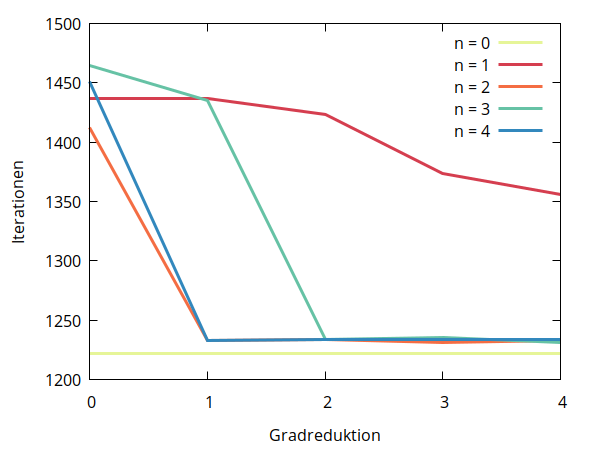
\includegraphics[width=\linewidth]{img/sweeping_only.png}  
  \caption{Sweeping beschränkt \textbf{square\_only}}
  \label{fig:sub1}
\end{subfigure}%
\begin{subfigure}{.5\textwidth}
  \centering
  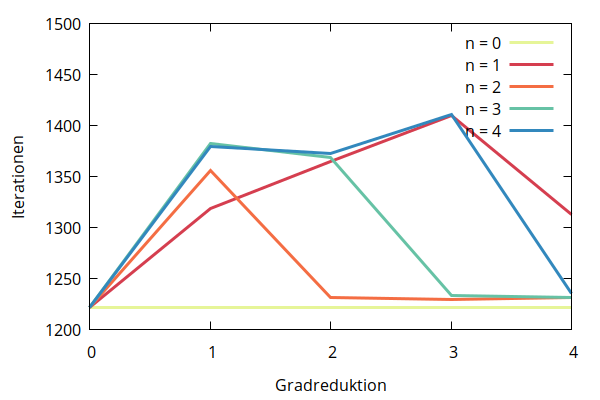
\includegraphics[width=\linewidth]{img/sweeping_first.png}
 \caption{Sweeping beschränkt \textbf{square\_first}}
  \label{fig:sub2}
\end{subfigure}

\begin{subfigure}{.5\textwidth}
  \centering
  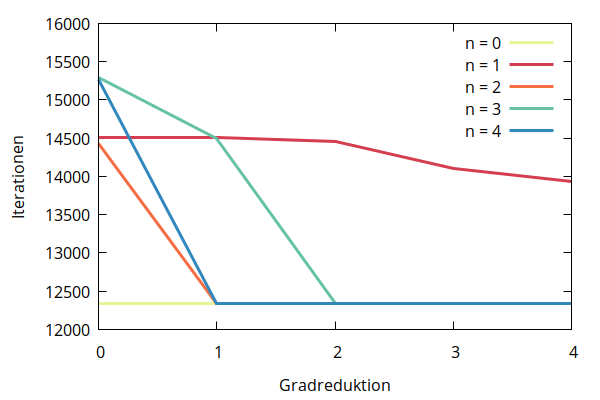
\includegraphics[width=\linewidth]{img/sweeping_only10k.png}
  \caption{Sweeping beschränkt \textbf{square\_only}}  
  \label{fig:sub1}
\end{subfigure}%
\begin{subfigure}{.5\textwidth}
  \centering
  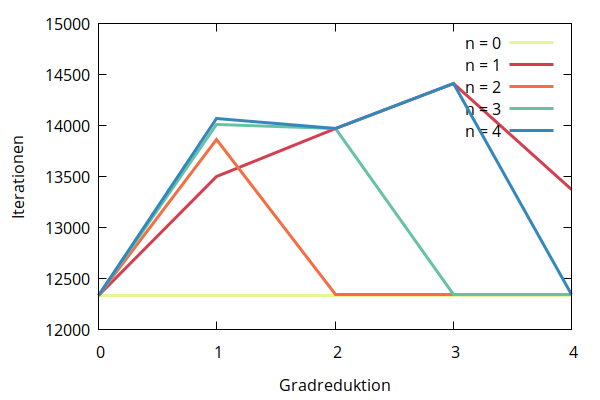
\includegraphics[width=\linewidth]{img/sweeping_first10k.png}
 \caption{Sweeping beschränkt \textbf{square\_first}}
  \label{fig:sub2}
\end{subfigure}
\caption[Sweeping mit verschiedenen Graden]{Anzahl an Iterationen mit Erhalt der n größten Fehlersymbole. (a) (b): 1000 Bits Präzision , $x_0 = y_0 = [0 \pm 2^{1000}]$.
 (c)(d): 10000 Bits Präzision , $x_0 = y_0 = [0 \pm 2^{10000}]$
}
\label{fig:sweeping}
\end{figure}

Im Vergleich mit rein linearen Taylormodellen zeigt sich eine Verbesserung (siehe Abbildung \ref{fig:extra}). Der Unterschied besteht darin, dass die nichtlinearen Taylormodelle während der Berechnung und besonders während der Multiplikation Punktintervalle erhalten können und sich stattdessen der Grad und die Länge des Polynoms erhöht. Nach jeder Iteration werden dann verschiedene Monome durch Gradreduktion vereint, wobei die Intervalle breiter werden. Im nächten Schritt wird der Grad dann durch Splitting auf den Monomen um maximal 1 erhöht und es liegen wieder Punktintervalle vor. Für lineare Taylormodelle steht lediglich das Splitting für den Kernel zur Verfügung, da sonst nichtlineare Polynome entstünden. Des Weiteren wird hier bereits während der Multiplikation gesweept und Punktintervalle werden zu regulären Intervallen. Die Performanz des Sweepings \textbf{square\_only} zum Grade 0 verbessert sich im Schnitt mit einer wachsenden Zahl der zu erhaltenen Fehlersymbole, wie in Abbildung \ref{fig:extra} zu sehen ist. Jedes Fehlersymbol erhöht die Menge an erhaltener Abhängigkeitsinformation und sorgt dafür, dass ein Taylormodell dessen Ränder besser beschreiben kann. Allerdings stellt die Praktikabilität dieser Herangehensweise ein Problem dar, da so sehr große Polynome entstehen, die während einer Iteration der H\e non-Abbildung exponentiell in ihrer Länge wachsen.
 

 \Abbildungps{tbh}{.7}{img/extra.png}{fig:extra}{Experimentelle Ergebnisse zu erhaltenen Fehlersymbolen}{Gegenüberstellung von $x_0 = y_0 = [0 \pm 2^{10000}]$ als lineare Taylormodelle und nichtlineare Taylormodelle mit quadratischem Sweeping zum Grade 0. Jeweils bleiben verschiedene Anzahlen von Fehlersymbolen pro Iteration erhalten. Gemessen wird die Iterationszahl der H\e non-Abbildung mit fester Genauigkeit von 10000 Bits, bis $|x_n|\cdot|y_n|$ einen Grenzwert von $2^{-6}$ überschreitet. }

 Dieser Effekt ist in Tabelle \ref{tab:time} verdeutlicht. Eine Erhöhung der Anzahl der erhaltenen Fehlersymbole hat einen drastischen Einfluss auf die durchschnittliche Dauer einer Iteration in $ms$, bis das Programm bei größeren Werten quasi nicht mehr lauffähig ist ($>100ms$ pro Iteration). Betrachtet man nun das Verhältnis zwischen der Verbesserung der Performanz (Abbildung \ref{fig:extra}) und der Verschlechterung der Laufzeit (Tabelle \ref{tab:time}), so bildet das Setzen der erhaltenen Fehlersymbole auf 3 mit einem Zielgrade von 0 bei der Beschränkung auf quadratisches Sweeping einen guten Trade-off, weshalb diese Konfiguration als Voreinstellung für Sweeping in der Implementierung (Kapiter \ref{ch:umsetung}) vorgesehen ist.
 
  
 \begin{table}[tbh]
\centering
\begin{tabular}{|c||c|c|c|c|c|}
\hline
&\multicolumn{5}{c|}{Erhaltene Fehlersymbole pro Iteration} \\
\hline
Gradreduktion & 0 & 1 &2& 3 & 4\\
\hline
0& 0.166& 0.603&    2.097&   4.358&    13.354\\
1& 0.166& 0.939&   2.358&  7.470&   >100\\
2& 0.166& 1.645&     5.750&   20.339 &    >100\\
3& 0.166& 2.284&     2.977&   74.172&    >100\\
4&0.166& 2.658&    3.622&   >100    &   >100\\
\hline 
&\multicolumn{5}{c|}{$ms$ pro Iteration} \\
\hline
\end{tabular}

\caption[Experimentelle Ergebnisse zu erhaltenen Fehlersymbolen]{Durchschnittliche Dauer einer Iteration der H\e non-Abbildung in $ms$ mit Taylormodelle der Größe $[0\pm 2^{-10000}]$ bei festgelegter Präzision von 10000 Bits und 1000 Iterationen.}
\label{tab:time}
\end{table}
 
 
 \section{Cleaning}
 Durch die mehrstufige Intervallstruktur in den Koeffizienten der Polynome ist es mit Cleaning möglich, den Rechenfehler, beziehungsweise die Intervallbreite der Intervallgrenzen auf einer höheren Abstraktionsebene zu verwalten. Wie in Paragraph \ref{par:cleaning} beschrieben, wird das Intervall um die Intervallbreite des Mittelpunktes und des Radius' erweitert und schließt es somit komplett ein. Dies hat darüber hinaus den Effekt, dass sämtlicher entstandene Rechenfehler durch Anwendung von Splitting reduziert werden kann. 
 
   \Abbildungps{tbh}{.7}{img/clean.png}{fig:clean}{Experimentelle Ergebnisse zum Effekt des Cleaning}{Iterationszahl der H\e non-Abbildung mit festem Radius der intialen Taylormodelle $x_0 = y_0 = [0 \pm 2^{-1000}]$ mit wachsender Präzision, um den Effekt des Cleanings beschreiben.}
 
 Abbildung \ref{fig:clean} zeigt die Auswirkung der Anwendung von Cleaning bei initialen Taylormodellen $x_0, y_0$ der Breite $2^{-1000}$ mit wachsender Genauigkeit. Cleaning sorgt für ein langsameres Wachstum des Rechtecks $|x_n|\cdot|y_n|$ nach $n$ Iterationen im Vergleich zur Berechnung ohne Cleaning. Bei einer höheren Anzahl der erhaltenen Fehlersymbole pro Iteration wird der Effekt noch deutlicher, da nun mit deutlich längeren Polynomen gerechnet und dementsprechend mehr arithmetische Operationen auf den Koeffizienten angewandt werden. So bleibt zwar mehr Information über Form der Taylormodelle erhalten, jedoch dominiert die Überschätzung auf der Zahlenebene das Ergebnis beim Verzicht auf Cleaning, während sich die Performanz im anderen Fall leicht verbessert.
 

 
 
 \section{Splitting}
 Durch Splitting wird ein Monom mit Intervallkoeffizienten in zwei Monome mit einem neuen, noch nicht verwendeten Fehlersymbol und Punktintervallkoeffizienten aufgeteilt. Für diese Housekeeping-Methode wurden zwei Möglichkeiten betrachtet. Zum Einen die in \cite{DBLP:conf/macis/BrausseKM15} verwendete Definition des neuen Fehlersymbols als Einheitsintervall:
 
\begin{align}
\label{int:unit}
 [c \pm \varepsilon]  \underset{split}{\rightsquigarrow} [c] + [\varepsilon] \cdot \lambda_{new}, \lambda_{new} \in [0 \pm 1]
\end{align}

Zum Anderen die Umlagerung des Radius $\varepsilon$ in das neue Fehlersymbol:

\begin{align}
\label{int:nunit}
 [c \pm \varepsilon]  \underset{split}{\rightsquigarrow} [c] + [1] \cdot \lambda_{new}, \lambda_{new} \in [0 \pm \varepsilon]
\end{align}
 
Beim Sweeping hat sich gezeigt, dass die Überschätzung des Taylormodells bei einer Priorisierung kleinerer Fehlersymbole, beziehungsweise durch Erhalt von Fehlersymbolen mit größerem Support-Space, langsamer wächst. In einer linearen Implementierung der Taylormodelle mit Variante \ref{int:unit} wird eine solche Ordnung durch einen Vergleich der Koeffizienten hergestellt, da jedes Monom maximal ein Fehlersymbol enthalten kann. Ein nichtlineares Monom kann jedoch von mehreren Fehlersymbolen abhängen, wodurch die Information über die Größe des Fehlersymobls nicht im Koeffizienten kodiert werden kann und zudem innerhalb eines Monoms sortiert werden muss. Daher eignet sich Herangehensweise \ref{int:nunit} für die Implementierung nichtlinearer Taylormodelle besser, als die Verwendung von Einheitsintervallen, wie in Abbildung \ref{fig:split} an einem Bespiel gezeigt wird. Hier werden beide Varianten auf die Entwicklung der Überschätzung von zwei Taylormodellen untersucht, wobei mit der Definition des Fehlersymbols als reguläres Intervall \ref{int:nunit} mehr Iterationen der H\e non-Abbildung berechnet werden können, bis die Fläche des Rechtecks einen Schwellenwert, wie oben überschreitet.
 
 \Abbildungps{tbh}{.7}{img/split.png}{fig:split}{Experimentelle Ergebnisse zum Vorgehen beim Splitting}{Iterationszahl der H\e non-Abbildung mit 10000 Bits fester Genauigkeit.}
 
 \section{Initiales Taylormodell}
 
 Für die H\e non-Abbildung wird ein Punkt $(x_0,y_0) \in \mathbb{R}^2$ wiederum in den $\mathbb{R}^2$ abgebildet. $x_0$ und $y_0$ können nun als Taylormodelle verschiedener Form definiert werden:
 
 
 \begin{align}
  &[c] + [1] \cdot \lambda,\  \lambda \in [0 \pm \varepsilon] \label{tm1}\\
  &[c] + [\varepsilon] \cdot \lambda,\ \lambda \in [0 \pm 1] \label{tm2}\\
  &[0] + [c \pm \varepsilon] \cdot \lambda,\ \lambda \in [1] \label{tm3}\\
  &[c \pm \varepsilon]\label{tm4} 
 \end{align}


Die verschiedenen Taylormodelle wurden verwendet, um die Intervalle $[0 \pm 2^{-1000}]$, beziehungsweise $[0\pm 2^{-10000}]$ in $x_0$ und $y_0$ darzustellen. Tabelle \ref{tab:tm} zeigt, wieviele Iterationen mit der jeweiligen Definition möglich sind, bis die Fläche des Rechtecks von $|x|\cdot|y|$ einen Schwellenwert überschreitet.
 
 
\begin{table}[tbh]
\centering
\begin{tabular}{|c||l|l||l|l|}
\hline
&\multicolumn{2}{c||}{1000 Bit Präzision} & \multicolumn{2}{c|}{10000 Bit Präzision} \\
\hline
Taylormodell & Iterationen & $|x| \cdot |y|$ &Iterationen & $|x| \cdot |y|$\\
\hline
TM \ref{tm1} & 1437 & 0.17 &14506 & 0.78 \\ 
TM \ref{tm2}  & 1227 & 0.49&12338 & 0.19  \\
TM \ref{tm3} & 1437 &  0.37&14505 & 0.17  \\                                                                 
TM \ref{tm4}  & 1437 & 0.35 &14505 & 0.18  \\
\hline 
\end{tabular}

\caption[Experimentelle Taylormodell Varianten]{Berechnung der Fläche des Rechtecks mit verschiedenen Definitionen der initialen Taylormodelle für $x$ und $y$ bei festgelegter Präzision.}
\label{tab:tm}
\end{table}
 
 
Bis auf Taylormodell-Definition \ref{tm2} erreichen (beinahe) alle Berechnung dieselbe Iterationszahl, variieren jedoch in der Größe des Rechtecks, welches von $x$ und $y$ aufgespannt wird. Mit der Definition \ref{tm1} als intiales Taylormodell wird für 10000 Bit Genauigkeit eine minimal höhere Iterationszahl und bei 1000 Bit Genauigkeit ein kleineres Rechteck, als in den anderen Varianten erreicht.
 
 \section{Anwendung der Parameter}
 \label{sec:anwendung}
 In diesem Kapitel wurden mit verschiedenen Belegungen für die zu Verfügung stehenden Parameter in $\verb+HOTM+$ versucht, eine möglichst optimale Konfiguration im Hinblick auf die Eindämmung der Überschätzung des Intervalls zu finden. Die besten Ergebnisse werden hierbei erzielt mit: 
 \begin{itemize}
  \item \textbf{Sweeping} mit ausschließlich quadratischem Sweeping zum Grade 0,
  \item \textbf{Cleaning} und \textbf{Splitting} mit einem Grenzwerten orientiert an der Genauigkeit,
  \item \textbf{Initialen Taylormodellen} für ein Intervall $[c \pm \varepsilon]$ der Form $[c] + [1] \cdot \lambda,\  \lambda \in [0 \pm \varepsilon]$,
  \item Erhalt von 3 \textbf{Fehlersymbolen}.
 \end{itemize}
Abbildung \ref{fig:lyapu_int_tm} zeigt die Entwicklung bei Berechnungen der H\e non-Abbildung. Jeweils zu sehen sind (1) der Abstand der $x$-Koordinate zweier Punkte $a=(0,0)$ und $b=(2^{-p},2^{-p})$ in Farbe, (2) die Breite des Intervalls $|x_n|$ für $(x_0, y_0)=([0\pm 2^{-(p-1)}],[0\pm 2^{-(p-1)}])$ in grau und (3) die Breite des ausgewerteten Taylormodells $|x_n|$ für zwei Taylormodelle $x_0 = [0] + [1]\cdot \lambda_0, \lambda_0\in [0\pm 2^{-(p-1)}]$ und $y_0 = [0] + [1]\cdot \lambda_1, \lambda_1\in [0\pm 2^{-(p-1)}]$ in schwarz. Der Verlauf der unabhängigen Punkte (1) stellt eine lokale Annäherung an den Lyapunov Exponenten dar und damit eine untere Schranke an die Ausbreitung eines Rechtecks pro Iteration der H\e non-Abbildung dar, indem sie dessen Eckpunkte markieren. Es ist deutlich erkennbar, dass sich das Taylormodell (3) langsamer ausbreitet und damit näher an der Schranke bewegt, als die Berechnung mit reiner Intervallartihmetik (2).
 
 
  \Abbildungps{tbh}{1}{img/lyapu_int_tm.png}{fig:lyapu_int_tm}{Vergleich der Entfernung von Punkten, eines Intervalls und eines Taylormodells}{Entwicklung des Abstandes der x-Koordinate zweier Punkte $(0,0)$ und $(\varepsilon,\varepsilon)$ in Farbe, der Breite des Intervalls des x-Wertes eines Rechtecks $([0\pm \varepsilon], [0\pm \varepsilon])$ in Grau und der Breite des ausgewerteten Taylormodells für die x-Koordinate in Schwarz mit $|x_0| = \varepsilon$. Getestet bei der H\e non-Iteration mit $a=1.4$ und $b=0.3$.}
 
 \newpage
 \section{Umsetzung}
 \label{ch:umsetung}
 Zwei Implementierungen der H\e non-Abbildung für die Parameter $a=1.4$ und $b=0.3$ sind in den Listings \ref{list:point} und \ref{list:int} zu sehen. Es werden drei verschiedenene Zahlentypen verwendet, die jedoch alle auf den \verb+iRRAM-REAL+s aufbauen: \textit{High Order Taylor Modell} \verb+HOTM+, \textit{Real Number} \verb+num+ und \textit{Real Number Interval} \verb+numint+. Die jeweils definierte Funktion \verb+compute()+ in Zeile 5 stellt den in der \verb+iRRAM+ verwendeten Rahmen für Iterationen, beziehungsweise Erhöhungen der Genauigkeit der \verb+REAL+s dar. Mit dem Funktionsaufruf \verb+HOTM::init()+ in Zeile 9 werden die zuvor in diesem Kapitel beschriebenen Grenzwerte und Parameter für die Housekeeping-Methoden mit Werten initialisiert, die experimentell die beste Performanz lieferten. Die Parameter $a$ und $b$ werden in Zeile 14 als \verb+num+ (\verb+iRRAM::REAL+) instanziiert. Die Durchführung der Housekeeping-Methoden ist ein Überschreiben des Zuweisungsoperators \anf{=} für die \verb+HOTM+-Taylormodelle realisiert. Während der Berechnung in den Zeilen 17 und 18 können sich die Taylormodelle aufblähen und werden dann bei der Zuweisung reduziert. In den Zeilen 19 und 20 findet kein Housekeeping mehr statt, gesteuert durch einen Parameter, der den Zustand des Taylormodells beschreibt \footnote{Operationen auf dem Taylormodell markieren es als \anf{not cleaned}. Dieser Wert wird dann durch die Anwendung von Housekeeping zurückgesetzt.}.
 
 
 \begin{minipage}{.5\textwidth}
    \begin{lstlisting}[language=C++, style=cpp, caption={[Implementierung der H\e non-Iteration in HOTM mit Punktintervallen] \\Implementierung mit Punktintervallen },label=list:point]
#include "iRRAM.h"
#include "hoTM.h"
using namespace iRRAM;

void compute(){
 int n;
 cin >> n;
 
 HOTM::init();
 HOTM x(num(0));
 HOTM y(num(0));
 HOTM x_new, y_new;
 
 num a(1.4), b(0.3);
 for (int i = 0; i < n; i++) {
 
   x_new = 1+y-a*(x*x);
   y_new = b*x;
   x = x_new;
   y = y_new;
 }
 cout<<"x:"<< numint(x) <<"\n";
 cout<<"y:"<< numint(y) <<"\n";
}
\end{lstlisting}
 \end{minipage}
 \begin{minipage}{.5\textwidth}
    \begin{lstlisting}[language=C++,  style=cpp, caption={[Implementierung der H\e non-Iteration in HOTM mit Intervallen] \\Implementierung mit Intervallen }, label=list:int]  
#include "iRRAM.h"
#include "hoTM.h"
using namespace iRRAM;

void compute(){
 int n;
 cin >> n;
 
 HOTM::init(2);
 HOTM x(num(0), num(0.001));
 HOTM y(num(0), num(0.001), 0);
 HOTM x_new, y_new;
 
 num a(1.4), b(0.3);
 for (int i = 0; i < n; i++) {
   HOTM::housekeep(x,y);
   x_new = 1+y-a*(x*x);
   y_new = b*x;
   x = x_new;
   y = y_new;
 }
 cout<<"x:"<< x <<"\n";
 cout<<"y:"<< y <<\n";
}
\end{lstlisting}
 \end{minipage}

 
 
 Um die Anpassung der Parameter der \verb+HOTM+ zu vereinfachen stehen verschiedene Möglichkeiten zur Verfügung:
 \paragraph{Initiale Taylormodelle}
 In der linken Implementierung \ref{list:point} werden $x$ und $y$ als Punktintervalle, also als Taylormodelle mit lediglich einem Kernel definiert:
  \begin{center}
  \verb+HOTM::x(0)+ $\rightsquigarrow x\coloneqq [0]$\\
  \verb+HOTM::y(0)+ $\rightsquigarrow y\coloneqq [0]$
 \end{center}

 
 Unter Verwendung des Konstruktors auf der rechten Seite wird aus der Eingabe eines Intervalls mit Mittelpunkt $c$ und Radius $\varepsilon$ je ein Taylormodell mit einem Fehlersymbol, welches $\varepsilon$ enthält und dem Kernel als Punktintervall $c$: 
 \begin{center}
  \verb+HOTM::x(0,0.001)+ $\rightsquigarrow x\coloneqq [0] + [1] \cdot \lambda_0,\ \lambda_0 \in [0 \pm 0.001]$\\
  \verb+HOTM::y(0,0.001)+ $\rightsquigarrow y\coloneqq[0] + [1] \cdot \lambda_1,\ \lambda_1 \in [0 \pm 0.001]$
 \end{center}

\paragraph{Anzahl der zu erhaltenden Fehlersymbole}
Die Initialisierungsfunktion \verb+init()+ akzeptiert eine \verb+int+ $\geq 0$ als Eingabe. Damit kann die Anzahl der zu erhaltenden Fehlersymbole pro Taylormodellangepasst werden, wie in  Listing \ref{list:int} Zeile 9. Der Standardwert liegt bei 3. Außerdem besteht die Möglichkeit, diesen Wert für jedes Taylormodell individuell zu bestimmen (Listing \ref{list:int} Zeile 11). Ist dieser Wert nicht gesetzt, so wird er aus dem \verb+init()+ Aufruf abgeleitet.

\paragraph{Manuelles Housekeeping}
 Sollen die Housekeeping-Methoden nur für bestimmte Taylormodelle oder zu einem anderen Zeitpunkt, als bei der Zuweisung durchgeführt werden, so wird die Funktion \verb+HOTM::kousekeep+ aufgerufen. Ein Aufruf, wie in Listing \ref{list:int} Zeile 16, schaltet das Housekeeping während der Zuweisung aus. Zudem wird das Entfernen bis auf die $m$-größten Fehlersymbole nun für alle im Aufruf enthaltenen Taylormodelle durchgeführt, statt einzeln. Das bedeutet, dass nach diesem Aufruf in allen Taylormodellen dieselben Fehlersymbole übrig bleiben.
 
\paragraph{Ausgabe}
 Die Ausgabe des Ergebnisses erfolgt jeweils in den Zeilen 22 und 23. Listing \ref{list:point} erzeugt hier eine Auswertung der Taylormodelle zu Intervallen mit einer Genauigkeit von 20 Stellen nach dem Komma für Mitte und Radius. In Listing \ref{list:int} hingegen werden die Taylormodelle aufgelistet, ohne diese auszuwerten. Das heißt, es werden alle Monome mitsamt ihrer Variablen angezeigt.
 

%%% Local Variables: 
%%% mode: latex
%%% TeX-master: "thesis"
%%% End: 
        % Evaluation  
%% zusammenf.tex
%% $Id: zusammenf.tex 61 2012-05-03 13:58:03Z bless $
%%

\chapter{Fazit}
\label{ch:fazit}
%% ==============================

\section{Diskussion}

\section{Ausblick}
In dieser Arbeit wurde eine grundlegende Implementierung für das Rechnen mit nichtlinearen Taylormodellen auf den reellen Zahlen beschrieben und angefertigt. An verschiedenen Stellen ist es jedoch möglich und teils notwendig, die Arbeit fortzuführen

\section{Partitionierung}

\section{Laufzeitoptimierung}

\section{Schnittstellen}


%%% Local Variables: 
%%% mode: latex
%%% TeX-master: "thesis"
%%% End: 
     % Diskussion und Ausblick

%% ++++++++++++++++++++++++++++++++++++++++++
%% Anhang
%% ++++++++++++++++++++++++++++++++++++++++++

\appendix
%\include{anhang_a}
%\include{anhang_b}

%% ++++++++++++++++++++++++++++++++++++++++++
%% Literatur
%% ++++++++++++++++++++++++++++++++++++++++++
%  mit dem Befehl \nocite werden auch nicht 
%  zitierte Referenzen abgedruckt

\cleardoublepage
\phantomsection
\addcontentsline{toc}{chapter}{\bibname}
%%
\nocite{*} % nur angeben, wenn auch nicht im Text zitierte Quellen 
           % erscheinen sollen
\bibliographystyle{itmabbrv} % mit abgekürzten Vornamen der Autoren
%\bibliographystyle{gerplain} % abbrvnat unsrtnat
% spezielle Zitierstile: Labels mit vier Buchstaben und Jahreszahl
%\bibliographystyle{itmalpha}  % ausgeschriebene Vornamen der Autoren
\bibliography{thesis}

\end{document}
%% end of file
